%%%%%%%%%%%%%%%%%%%%%%%%%%%%%%%%%%%%%%%%%
% University Assignment Title Page 
% LaTeX Template
% Version 1.0 (27/12/12)
%
% This template has been downloaded from:
% http://www.LaTeXTemplates.com
%
% Original author:
% WikiBooks (http://en.wikibooks.org/wiki/LaTeX/Title_Creation)
%
% License:
% CC BY-NC-SA 3.0 (http://creativecommons.org/licenses/by-nc-sa/3.0/)
% 
% Instructions for using this template:
% This title page is capable of being compiled as is. This is not useful for 
% including it in another document. To do this, you have two options: 
%
% 1) Copy/paste everything between \begin{document} and \end{document} 
% starting at \begin{titlepage} and paste this into another LaTeX file where you 
% want your title page.
% OR
% 2) Remove everything outside the \begin{titlepage} and \end{titlepage} and 
% move this file to the same directory as the LaTeX file you wish to add it to. 
% Then add %%%%%%%%%%%%%%%%%%%%%%%%%%%%%%%%%%%%%%%%%
% University Assignment Title Page 
% LaTeX Template
% Version 1.0 (27/12/12)
%
% This template has been downloaded from:
% http://www.LaTeXTemplates.com
%
% Original author:
% WikiBooks (http://en.wikibooks.org/wiki/LaTeX/Title_Creation)
%
% License:
% CC BY-NC-SA 3.0 (http://creativecommons.org/licenses/by-nc-sa/3.0/)
% 
% Instructions for using this template:
% This title page is capable of being compiled as is. This is not useful for 
% including it in another document. To do this, you have two options: 
%
% 1) Copy/paste everything between \begin{document} and \end{document} 
% starting at \begin{titlepage} and paste this into another LaTeX file where you 
% want your title page.
% OR
% 2) Remove everything outside the \begin{titlepage} and \end{titlepage} and 
% move this file to the same directory as the LaTeX file you wish to add it to. 
% Then add %%%%%%%%%%%%%%%%%%%%%%%%%%%%%%%%%%%%%%%%%
% University Assignment Title Page 
% LaTeX Template
% Version 1.0 (27/12/12)
%
% This template has been downloaded from:
% http://www.LaTeXTemplates.com
%
% Original author:
% WikiBooks (http://en.wikibooks.org/wiki/LaTeX/Title_Creation)
%
% License:
% CC BY-NC-SA 3.0 (http://creativecommons.org/licenses/by-nc-sa/3.0/)
% 
% Instructions for using this template:
% This title page is capable of being compiled as is. This is not useful for 
% including it in another document. To do this, you have two options: 
%
% 1) Copy/paste everything between \begin{document} and \end{document} 
% starting at \begin{titlepage} and paste this into another LaTeX file where you 
% want your title page.
% OR
% 2) Remove everything outside the \begin{titlepage} and \end{titlepage} and 
% move this file to the same directory as the LaTeX file you wish to add it to. 
% Then add %%%%%%%%%%%%%%%%%%%%%%%%%%%%%%%%%%%%%%%%%
% University Assignment Title Page 
% LaTeX Template
% Version 1.0 (27/12/12)
%
% This template has been downloaded from:
% http://www.LaTeXTemplates.com
%
% Original author:
% WikiBooks (http://en.wikibooks.org/wiki/LaTeX/Title_Creation)
%
% License:
% CC BY-NC-SA 3.0 (http://creativecommons.org/licenses/by-nc-sa/3.0/)
% 
% Instructions for using this template:
% This title page is capable of being compiled as is. This is not useful for 
% including it in another document. To do this, you have two options: 
%
% 1) Copy/paste everything between \begin{document} and \end{document} 
% starting at \begin{titlepage} and paste this into another LaTeX file where you 
% want your title page.
% OR
% 2) Remove everything outside the \begin{titlepage} and \end{titlepage} and 
% move this file to the same directory as the LaTeX file you wish to add it to. 
% Then add \input{./title_page_1.tex} to your LaTeX file where you want your
% title page.
%
%%%%%%%%%%%%%%%%%%%%%%%%%%%%%%%%%%%%%%%%%
%\title{Title page with logo}
%----------------------------------------------------------------------------------------
%	PACKAGES AND OTHER DOCUMENT CONFIGURATIONS
%----------------------------------------------------------------------------------------

\documentclass[12pt]{article}
\usepackage[english]{babel}
\usepackage[utf8x]{inputenc}
\usepackage{amsmath}
\usepackage{graphicx}
\usepackage{listings}
\usepackage{color}
\usepackage{xcolor}
\usepackage{amssymb}
\usepackage{hyperref}
\usepackage{pdfpages}


\definecolor{dkgreen}{rgb}{0,0.6,0}
\definecolor{gray}{rgb}{0.5,0.5,0.5}
\definecolor{mauve}{rgb}{0.58,0,0.82}

\lstset{frame=tb,
	language=C,
	aboveskip=3mm,
	belowskip=3mm,
	showstringspaces=false,
	columns=flexible,
	basicstyle={\small\ttfamily},
	numbers=none,
	numberstyle=\tiny\color{gray},
	keywordstyle=\color{blue},
	commentstyle=\color{dkgreen},
	stringstyle=\color{mauve},
	breaklines=true,
	breakatwhitespace=true,
	tabsize=3
}

\makeatletter
\newsavebox\myboxA
\newsavebox\myboxB
\newlength\mylenA

\newcommand*\xoverline[2][0.75]{%
	\sbox{\myboxA}{$\m@th#2$}%
	\setbox\myboxB\null% Phantom box
	\ht\myboxB=\ht\myboxA%
	\dp\myboxB=\dp\myboxA%
	\wd\myboxB=#1\wd\myboxA% Scale phantom
	\sbox\myboxB{$\m@th\overline{\copy\myboxB}$}%  Overlined phantom
	\setlength\mylenA{\the\wd\myboxA}%   calc width diff
	\addtolength\mylenA{-\the\wd\myboxB}%
	\ifdim\wd\myboxB<\wd\myboxA%
	\rlap{\hskip 0.5\mylenA\usebox\myboxB}{\usebox\myboxA}%
	\else
	\hskip -0.5\mylenA\rlap{\usebox\myboxA}{\hskip 0.5\mylenA\usebox\myboxB}%
	\fi}
\makeatother

\begin{document}

\begin{titlepage}

\newcommand{\HRule}{\rule{\linewidth}{0.5mm}} % Defines a new command for the horizontal lines, change thickness here

\center % Center everything on the page
 
%----------------------------------------------------------------------------------------
%	HEADING SECTIONS
%----------------------------------------------------------------------------------------

\textsc{\LARGE Politecnico di Milano}\\[1.5cm] % Name of your university/college
\textsc{\Large Dipartimento di Elettronica, Informazione e Bioingegneria}\\[0.5cm] % Major heading such as course name
\textsc{\large HEAPLab Project Report}\\[0.5cm] % Minor heading such as course title

%----------------------------------------------------------------------------------------
%	TITLE SECTION
%----------------------------------------------------------------------------------------

\HRule \\[0.4cm]
{ \huge \bfseries Floating Point Predictability}\\[0.4cm] % Title of your document
\HRule \\[1.5cm]
 
%----------------------------------------------------------------------------------------
%	AUTHOR SECTION
%----------------------------------------------------------------------------------------

\begin{minipage}{0.4\textwidth}
\begin{flushleft} \large
\emph{Authors:}\\
Alessio \textsc{Cantina}\\ % Your name
Simone \textsc{Crippa}
\end{flushleft}
\end{minipage}
~
\begin{minipage}{0.5\textwidth}
\begin{flushright} \large
\emph{Supervisor:} \\
Dr. Federico \textsc{Reghenzani} % Supervisor's Name
\end{flushright}
\end{minipage}\\[1cm]

% If you don't want a supervisor, uncomment the two lines below and remove the section above
%\Large \emph{Author:}\\
%John \textsc{Smith}\\[3cm] % Your name

%----------------------------------------------------------------------------------------
%	DATE SECTION
%----------------------------------------------------------------------------------------

{\large \today}\\[2cm] % Date, change the \today to a set date if you want to be precise

%----------------------------------------------------------------------------------------
%	LOGO SECTION
%----------------------------------------------------------------------------------------


\includegraphics[width=100pt]{heaplogo.pdf}\\[1cm] % Include a department/university logo - this will require the graphicx package
 
%----------------------------------------------------------------------------------------

\vfill % Fill the rest of the page with whitespace

\end{titlepage}




\begin{abstract}
\textcolor{red}{Your abstract. - Summarize your work.}

This project aims to investigate floating point vs fixed point predictability.

To achieve this result, we have used 6 Worst Case Execution Time (WCET) benchmarks which involve a large number of floating point instructions.
We converted these benchmarks using only fixed point variables and then we added the logic to obtain multiple measurements.

Finally, we computed and analysed 8 statistics to find out if floating point operations or fixed point operations are more predictable.

\end{abstract}

\section{Introduction}

\textcolor{red}{Your introduction goes here! Some examples of commonly used commands and features are listed below, to help you get started.}

In this section we describe the devices used for the benchmarks and all the commands used to process the benchmarks.

\subsection{Devices used}

To have a better view of the problem, we decided to get samples from devices with different architecture.
In this project, we considered 3 architectures and 6 devices.\newline 
armv7l devices:
\begin{itemize}
	\item Device name: Freescale i.MX 6 Quad. Processor configuration: 4x Cortex-A9 @ 1.2 GHz
	\item Device name: ODROID-XU3. Processor name: Exynos 5422. Processor configuration: big.LITTLE 8 cores, 4x Cortex-A15 @ 2.0 GHz, 4x Cortex-A7 @ 1.4 GHz 
\end{itemize}
armv8a devices:
\begin{itemize}
	\item Device name: Xiaomi Mi 5s. Processor name: Snapdragon 821 (MSM8996). Processor configuration: big.LITTLE 4 cores: 2x Kryo @ 2.15 GHz, 2x Kryo @ 1.6 GHz
	\item Device name: Xiaomi Mi Mix 2. Processor name: Snapdragon 835 (MSM8998). Processor configuration: big.LITTLE 8 cores: 4x Kryo @ 2.45 GHz, 4x Kryo @ 1.9 GHz
\end{itemize}
x86\_64 devices:
\begin{itemize}
	\item Device name: Dell XPS 13 9360. Processor name: Intel i5 8250U. Processor configuration: 4 cores (8 threads) @ 3.40 GHz
	\item Device name: Dell Vostro 15 3568. Processor name: Intel i5 7200U.
	Processor configuration: 2 cores (4 threads) @ 3.10 GHz
\end{itemize}
\subsection{Compiling commands}

\begin{itemize}
	\item Compile a floating point benchmark: \begin{verbatim}gcc -o "output_name" "benchmark_name"\end{verbatim}
	\item Cross-compile a benchmark, useful to execute a benchmark on a smartphone with ARM processor: \begin{verbatim}arm-linux-gnueabi-gcc -static -march="arm_platform" -o 
	"output_name" "benchmark_name"\end{verbatim}
	\item To compile a fixed point benchmark remember to append at the end of the command the library used for fixed point operations: \begin{verbatim}fixed_op_64bit.c\end{verbatim}
\end{itemize}


\subsection{make commands}

A makefile has been produced so that make can be used to compile and execute all the benchmarks at once:

\begin{itemize}
	\item Initialize the project directory with support folders:\begin{verbatim}make init\end{verbatim}
	\item Compile all the benchmarks: \begin{verbatim}make\end{verbatim}
	\item Execute all the benchmarks: \begin{verbatim}make run\end{verbatim}
	\item Clear the project directory: \begin{verbatim}make clean\end{verbatim}
\end{itemize}

Note: the makefile supports gcc compilation as is, but it needs to be modified for cross compilation. Detailed instructions are available inside the makefile.

\subsection{Additional commands}

These commands are used to run benchmarks with a stress test running on the CPU cache

\begin{itemize}
	\item Stress the CPU cache on a specific set of CPUs:\begin{verbatim}taskset -c cpu_list stress-ng --cache N \end{verbatim} where cpu\_list is the select cluster (start\_CPU - end\_CPU) and N is the number of worker threads (1 thread for each CPU core)
	\item Execute the benchmarks on a specific set of CPUs: \begin{verbatim}taskset -c cpu_list\end{verbatim}
\end{itemize}

\section{Design and Implementation}

\subsection{Benchmarks}

To investigate this issue, we selected 6 floating point benchmarks from \href{http://www.mrtc.mdh.se/projects/wcet/benchmarks.html}{mrtc.mdh.se}.
These are the selected benchmarks:
\begin{enumerate}
	\item \textbf{ludcmp}: implementation of the \href{https://en.wikipedia.org/wiki/LU_decomposition}{LU decomposition} algorithm
	\item \textbf{minve}r: inversion of a floating point matrix
	\item \textbf{qsort\_exam}: non-recursive implementation of quick sort algorithm
	\item \textbf{qurt}: root computation of quadratic equations
	\item \textbf{select}: function to select the ${N}^{th}$ largest number in a floating point array
	\item \textbf{sqrt}: square root function implemented by Taylor series
\end{enumerate}

Since there is no automatic way in C to convert floating point operations into fixed point, we have defined rules to convert floating point benchmarks into fixed points.
\begin{enumerate}
	\item Convert all the floating values into fixed point values in a fair way, keeping the same variable dimension:
	\begin{itemize}
		\item float $\rightarrow$ int32\_t	
		\item double $\rightarrow$ int64\_t
	\end{itemize}
	\item Multiply every floating point value by ${2}^{SHIFT\_AMOUNT}$, where SHIFT\_AMOUNT defines the precision of the fixed point values.
	\item Convert every multiplication and division into the corresponding fixed point function:
	\begin{itemize}
		\item multiplication $\rightarrow$ fixed\_mul\_64bit	
		\item division $\rightarrow$ fixed\_div\_64bit
	\end{itemize}
\end{enumerate}

Moreover, all benchmarks are executed on random generated numbers, except qurt which computes multiple times the inversion of a matrix.\newline
Note: random numbers are generated setting a common seed using the \textit{srand()} function, so that every benchmark in its floating and fixed version works on the same values.
\subsection{Sampling of the benchmarks}

Original benchmarks have no built-in method to obtain the elapsed execution time. We have implemented and integrated in C a function which randomly generates arguments for the benchmark and measures the elapsed time.
Measurements are stored in text files for future analysis.

This is an example of the main function:
\begin{itemize}
	\item srand() is used to generate random numbers, using a seed to keep track of generated numbers.
	\item EXEC\_NUM is a constant which regulates the number of samples generated. In our case, we generate 100.000 samples.
	\item function\_to\_call(val) is the benchmark function with the argument.
	\item diff(timespec,timespec) is a support function which makes the difference between two time instants.
	\item CLOCK\_MONOTONIC\_RAW is used to get the time instant from the system without alterations (even from ntp)
	\item SHIFT\_AMOUNT is used to convert floating point values into fixed points, an higher SHIFT\_AMOUNT means an higher decimal precision.
\end{itemize}
\begin{lstlisting}
int main()
{
	struct timespec start,end;
	FILE * fp;
	fp = fopen ("benchmark_results.txt","w");
	int64_t val;
	srand(5);
	for (int i=0; i< EXEC_NUM ; i++){
		//convert float to int64 only if the benchmark is fixed point, if not no conversion is done
		val = (int64_t)((((rand() % 10000) / 100) - 50) * pow(2,SHIFT_AMOUNT));
		
		clock_gettime(CLOCK_MONOTONIC_RAW, &start);
		function_to_call(val);
		clock_gettime(CLOCK_MONOTONIC_RAW, &end);
		
		fprintf (fp, "%lld\n",(long long)(diff(start,end).tv_sec * pow(10,9))+(long long)diff(start,end).tv_nsec);
	}
	
	fclose (fp);
	return 0;
}
\end{lstlisting}

\subsection{Fixed point operations}

To support fixed point operations we had to introduce a shift amount, so that floating point numbers can be represented as integers with a fixed precision, given by the shift amount.\newline
Since we have analysed different architectures we had to take into account the limitations of the selected architectures.
x86\_64 have the support for 128-bit variables, which are necessary to compute multiplications and divisions. Instead, ARM architectures have no support for 128-bit variables, so we implemented a support library to handle this discrepancy.
The library automatically select the operations by checking if the architecture support 128-bit integers, if there is no support, the benchmark will use a portable implementation of multiplication and division which are based on 64-bit integers.\newline
Our implementation of fixed division and multiplication works with a variable shift amount, in our benchmarks we have always used a shift amount of 30 because in our scenario it allows to have the necessary precision.\newline
Note: to guarantee fairness we use hard-coded values for constants in benchmarks that are shifted by 30-bits, even though operations supports dynamical shift amounts these values have to be modified to comply with the new selected shift amount.\newline

\textbf{fixed\_div for 128-bit support}

\begin{lstlisting}
int64_t fixed_div_64(int64_t x, int64_t y, int shift_amount)
{
    return ((((__int128)x << shift_amount) / y));
}
\end{lstlisting}

\textbf{fixed\_mul for 128-bit support}

\begin{lstlisting}
int64_t fixed_mul_64(int64_t x, int64_t y, int shift_amount)
{
	return (int64_t)((((__int128)x * (__int128)y)) >> shift_amount);
}
\end{lstlisting}

\textbf{fixed\_div without 128-bit support}\newline
To implement the divison mantaining the 128 bit precision needed during the divison operation,  the dividend is splitted into two 64 bit integers. Then the divison is perfomed using the technique that can be found at this \href{https://codereview.stackexchange.com/questions/67962/mostly-portable-128-by-64-bit-division}{link}.\newline

\textbf{fixed\_mul without 128-bit support}\newline
To implement the multiplication mantaining the 128 bit precision needed during the multiplication operation,  the two factors are splitted into two 64 bit integers each. Then the multiplication is perfomed using the technique that can be found at this \href{https://stackoverflow.com/questions/31652875/fastest-way-to-multiply-two-64-bit-ints-to-128-bit-then-to-64-bit}{link}.



\subsection{Statistics used}
To compare floating point results to fixed point results we computed through a Python script 8 metrics useful to analyse the predictability of a benchmark.

\begin{enumerate}
	\item Minimum execution time, computed through the Python built-in function \textit{min()}
	\item Maximum execution time, computed through the Python built-in function \textit{max()}
	\item Sample mean, computed through the Python module numpy as \textit{numpy.mean()}, the formula is: $$\xoverline[0.8]{x} = \frac{X_1 + X_2 + \cdots + X_n}{n}
	= \frac{1}{n}\sum_{i}^{n} X_i$$
	\item Sample variance, computed through the Python module numpy as \textit{numpy.var()}, the formula is:$${s}^{2} = \frac{\sqrt{\sum_{i}^{n} {(x_i - \xoverline[0.8]{x})}^{2}}}{n-1}$$
	\item Sample standard deviation, computed through the Python module statistics as \textit{statistics.stdev()}, the formula is:
	$$s = \frac{\sqrt{\sum_{i}^{n} (x_i - \xoverline[0.8]{x})}}{n-1}$$
	\item KPSS test statistic, computed through the Python module statsmodels as \textit{statsmodels.tsa.stattools.kpss()}, the formula is:$$S = \frac{{T}^{-2}\sum_{t=1}^{T} {\hat{S}_t}^{2}}{\sigma_\epsilon}$$
	Where:
	\begin{itemize}
		\item T is the sample size
		\item ${\sigma_\epsilon}$ is the long-run variance
		\item ${\hat{S}_t} = \sum_{i}^{t}e(t)$ is the partial sum of the errors of the regression $y(t)$
	\end{itemize}
	\item BDS test statistic, computed through the Python module statsmodels as \textit{statsmodels.tsa.stattools.bds()}, the formula is: $$BDS_{\epsilon,m} = \frac{\sqrt{N}[C_{\epsilon,m}-{(C_{\epsilon,1})}^{m}]}{\sqrt{V_{\epsilon,m}}}$$
	Where:
	\begin{itemize}
		\item $C_{\epsilon,m} = \frac{1}{N_m(N_m-1)}\sum_{i\not=j}{I_{i,j;\epsilon}}$\\[0.1cm]
		Where:
		\begin{itemize}
			\item m is the number of embedding dimensions, used to embed the time series into m-dimensional vectors.
			\item ${I_{i,j;\epsilon}} = 1 \;\; if ||{x}^{m}_i - {x}^{m}_j|| <= \epsilon  \;\; = 0 \;\; otherwise$
		\end{itemize}
		
		\item $V_{\epsilon,m} = 4[{K}^{m} + 2\sum_{j=1}^{m-1}{K}^{m-j}{C}^{2j}_\epsilon + {(m-1)}^{2}{C}^{2m}_\epsilon - {m}^{2}K{C}^{2m-2}_\epsilon]$
		Where:
		\begin{itemize}
			\item $K=K_\epsilon = \frac{6}{N_m(N_m-1)*(N_m-2)}\sum_{i<j<N}h_{i,j,N;\epsilon}$
			\item $h_{i,j,N;\epsilon} = \frac{[I_{i,j;\epsilon}I_{j,N;\epsilon}+I_{i,N;\epsilon}I_{N,j;\epsilon}+I_{j,i;\epsilon}I_{i,N;\epsilon}]}{3}$
		\end{itemize}
	\end{itemize}
	We know under some hypothesis, that the quantity $[C_{\epsilon,m}-{(C_{\epsilon,1})}^{m}]$ can be considered as an asymptotic normal distribution with zero mean and variance $V_{\epsilon,m}$
	\item Hurst exponent, computed through the Python module hurst as \textit{compute\_Hc(array, kind='change', simplified=True)}, the formula is:\newline
	$\operatorname{E} \left [ \frac{R(n)}{S(n)} \right ]=C n^H  \text{  as } n \to \infty  \, $
	\newline Where:
	\begin{itemize}
		\item $R(n)$ is the range of the first n cumulative deviations from the mean, and $s(n)$ is their standard deviation
		\item $\operatorname{E} \left [x \right ] \,$ is the expected value
		\item n is the time span of the observation (number of data points in a time series)
		\item C is a constant.
	\end{itemize}
\end{enumerate}

We are interested in execution time predictability, so we need to compare how much the measurements are spread through sample standard deviation and sample variance.
\href{http://debis.deu.edu.tr/userweb//onder.hanedar/dosyalar/kpss.pdf}{KPSS} test statistic is a one tailed test, which indicates if the time series is stationary around a mean or a linear trend. A stationary time series have constant statistical properties (like mean and variance) over time.
\begin{itemize}
	\item Null hypothesis: the data is stationary
	\item Alternative hypothesis: the data is not stationary
\end{itemize}
Instead, \href{https://www.researchgate.net/publication/46554708_A_Fast_Algorithm_for_the_BDS_Statistic}{BDS} statistic is a double tailed test, which indicates if the time series is serial dependent.
\begin{itemize}
 	\item Null hypothesis: the data is independently and identically distributed (I.I.D.)
 	\item Alternative hypothesis: the data is not I.I.D.
\end{itemize}

Since BDS test statistic complexity increase with the sample size, it can't be done on all the samples at once, instead we compute it using a sliding window on the samples and then select the maximum BDS obtained.\newline
Hurst Exponent is used to measure the long-term memory of a time series:
\begin{enumerate}
	\item If the Hurst Exponent is in the 0.5-1 range, we have a time series with long-term positive autocorrelation, meaning that an high value in the series will be followed by another high value and also the future values will tend to be high.
	\item If the Hurst Exponent is in the 0-0.5 range, we have a time series with long-term switching between high and low values so a single high value will probably be followed by a low value and also the future values will keep this tendency to switch between high and low values.
	\item If the Hurst Exponent is equal to 0.5, we have 2 different scenarios:
	\begin{itemize}
		\item A completely uncorrelated series
		\item A time series with alternating positive and negative autocorrelation but the absolute values of the autocorrelation decay exponentially to zero.
	\end{itemize}
\end{enumerate}



\section{Experimental Results}
Now a series of histrograms are displayed to better comprehend the behaviour of the different architectures.
These histrograms show the standard deviation expressed in microseconds for each benchmark and each processor.
Note: that the x scale is logaritmic.\newline

\textbf{Intel x86\_64 histogram}\newline
\hspace*{-3.2cm}
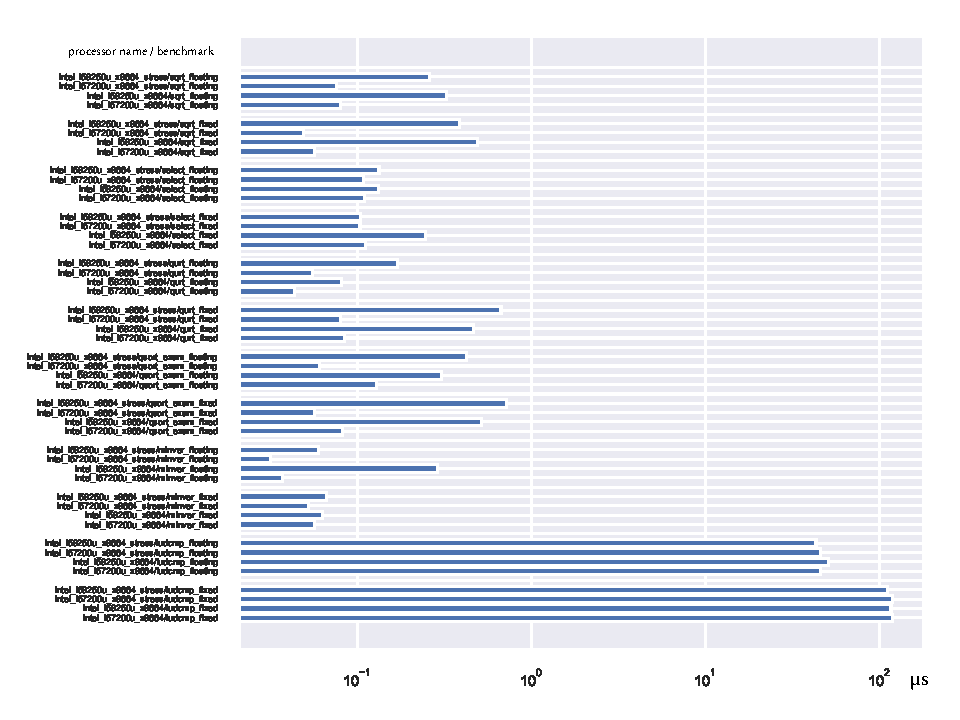
\includegraphics[width=570pt]{intel_histogram.pdf}
\clearpage
In the previous histogram we can identify the following singularities:
Comparing fixed point vs floating point operations:
\begin{itemize}
		\item In the benchmarks \textit{select}, \textit{qurt}, \textit{ludcmp} fixed point operations have a larger standard deviation.
		\item In the benchmarks \textit{sqrt}, \textit{qsort\_exam}, \textit{minver} we observe conflicting behaviours between the two processors (ex: in the \textit{qsort\_exam} benchmark the Intel i5 7200U has a lower standard deviation for the fixed point benchamark with respect to the floating point one. Instead the Intel i5 8250U has the opposite behaviour).
\end{itemize}
Comparing fixed point vs floating point operations with stress:
\begin{itemize}
		\item In the benchmarks \textit{qurt}, \textit{minver}, \textit{ludcmp} fixed point operations have a larger standard deviation.
		\item In the benchmark \textit{select} fixed point operations have a smaller standard deviation.
		\item In the benchmarks \textit{sqrt}, \textit{qsort\_exam} we observe conflicting behaviours between the two processors.
\end{itemize}

\clearpage
\textbf{Smartphones ARMv8a histogram}\newline
\hspace*{-3.2cm}
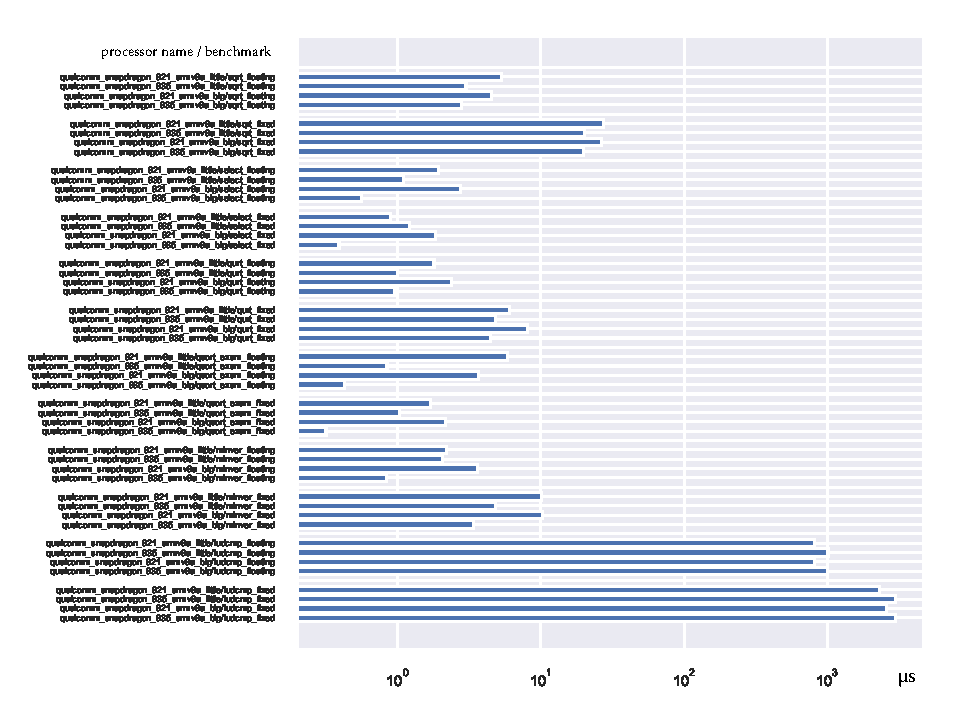
\includegraphics[width=570pt]{smartphones_histogram.pdf}
\clearpage
In the previous histogram we can identify the following singularities:
Comparing fixed point vs floating point operations on the big cluster:
\begin{itemize}
		\item In the benchmarks \textit{sqrt}, \textit{qurt}, \textit{minver}, \textit{ludcmp} fixed point operations have a larger standard deviation.
		\item In the benchmarks \textit{select}, \textit{qsort\_exam} fixed point operations have a smaller standard deviation.
\end{itemize}
Comparing fixed point vs floating point operations on the LITTLE cluster:
\begin{itemize}
		\item In the benchmarks \textit{sqrt}, \textit{qurt}, \textit{minver}, \textit{ludcmp} fixed point operations have a larger standard deviation.
		\item In the benchmarks \textit{select}, \textit{qsort\_exam} we observe conflicting behaviours between the two processors.
\end{itemize}

\clearpage
\textbf{Freescale IMX6 and Odroid XU3 histogram}\newline
\hspace*{-3.2cm}
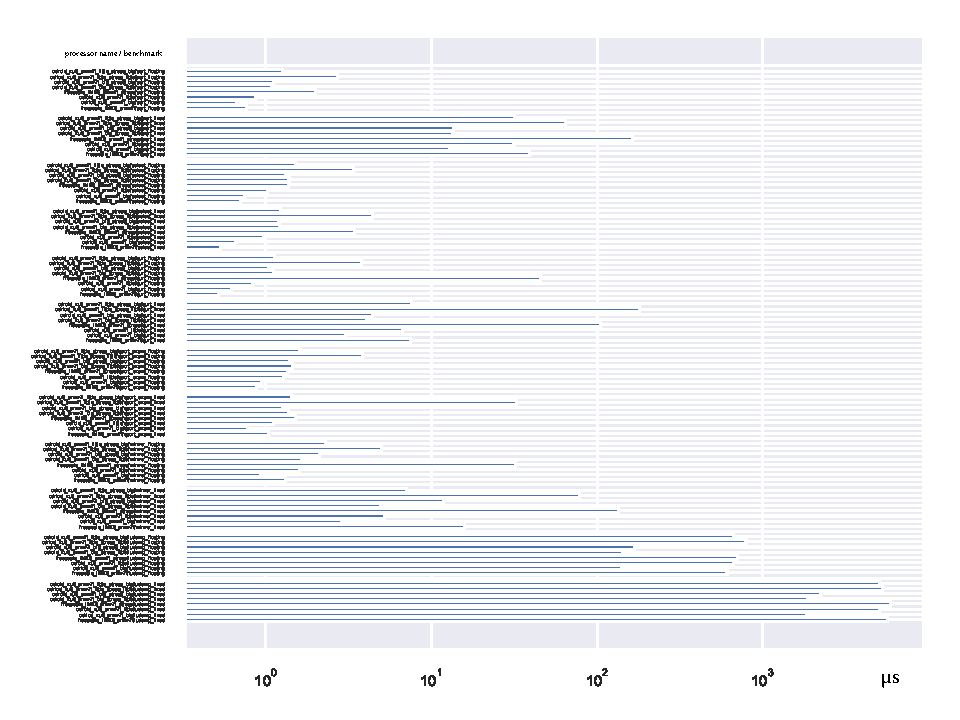
\includegraphics[width=570pt]{boards_histogram.pdf}
\clearpage
In the previous histogram we can identify the following singularities:
Comparing fixed point vs floating point operations on the Freescale IMX6 and the Odroid XU3 big and LITTLE cluster:
\begin{itemize}
		\item In the benchmarks \textit{sqrt}, \textit{qurt}, \textit{minver}, \textit{ludcmp} fixed point operations have a larger standard deviation.
		\item In the benchmark \textit{select} fixed point operations have a smaller standard deviation.
		\item In the benchmark \textit{qsort\_exam} we observe conflicting behaviours between the two processors (Odroid XU3 has lower standard deviation for fixed point operations, Freescale IMX6 has an higher standard deviation).
\end{itemize}
Comparing fixed point vs floating point operations with stress on the Freescale IMX6 and the Odroid XU3 big and LITTLE cluster:
\begin{itemize}
		\item In the benchmarks \textit{sqrt}, \textit{qurt}, \textit{minver}, \textit{ludcmp} fixed point operations have a larger standard deviation.
		\item In the benchmarks \textit{select}, \textit{qsort\_exam} we observe conflicting behaviours between the two processors (In the \textit{select} benchmark the Odroid XU3 running on the LITTLE cluster and stressed on this cluster has a higher standard deviation, the same for the Freescale IMX6 under stress. The exact same behaviour is observed with the benchmark \textit{qsort\_exam}).
\end{itemize}

\section{Conclusions}

\end{document} to your LaTeX file where you want your
% title page.
%
%%%%%%%%%%%%%%%%%%%%%%%%%%%%%%%%%%%%%%%%%
%\title{Title page with logo}
%----------------------------------------------------------------------------------------
%	PACKAGES AND OTHER DOCUMENT CONFIGURATIONS
%----------------------------------------------------------------------------------------

\documentclass[12pt]{article}
\usepackage[english]{babel}
\usepackage[utf8x]{inputenc}
\usepackage{amsmath}
\usepackage{graphicx}
\usepackage{listings}
\usepackage{color}
\usepackage{xcolor}
\usepackage{amssymb}
\usepackage{hyperref}
\usepackage{pdfpages}


\definecolor{dkgreen}{rgb}{0,0.6,0}
\definecolor{gray}{rgb}{0.5,0.5,0.5}
\definecolor{mauve}{rgb}{0.58,0,0.82}

\lstset{frame=tb,
	language=C,
	aboveskip=3mm,
	belowskip=3mm,
	showstringspaces=false,
	columns=flexible,
	basicstyle={\small\ttfamily},
	numbers=none,
	numberstyle=\tiny\color{gray},
	keywordstyle=\color{blue},
	commentstyle=\color{dkgreen},
	stringstyle=\color{mauve},
	breaklines=true,
	breakatwhitespace=true,
	tabsize=3
}

\makeatletter
\newsavebox\myboxA
\newsavebox\myboxB
\newlength\mylenA

\newcommand*\xoverline[2][0.75]{%
	\sbox{\myboxA}{$\m@th#2$}%
	\setbox\myboxB\null% Phantom box
	\ht\myboxB=\ht\myboxA%
	\dp\myboxB=\dp\myboxA%
	\wd\myboxB=#1\wd\myboxA% Scale phantom
	\sbox\myboxB{$\m@th\overline{\copy\myboxB}$}%  Overlined phantom
	\setlength\mylenA{\the\wd\myboxA}%   calc width diff
	\addtolength\mylenA{-\the\wd\myboxB}%
	\ifdim\wd\myboxB<\wd\myboxA%
	\rlap{\hskip 0.5\mylenA\usebox\myboxB}{\usebox\myboxA}%
	\else
	\hskip -0.5\mylenA\rlap{\usebox\myboxA}{\hskip 0.5\mylenA\usebox\myboxB}%
	\fi}
\makeatother

\begin{document}

\begin{titlepage}

\newcommand{\HRule}{\rule{\linewidth}{0.5mm}} % Defines a new command for the horizontal lines, change thickness here

\center % Center everything on the page
 
%----------------------------------------------------------------------------------------
%	HEADING SECTIONS
%----------------------------------------------------------------------------------------

\textsc{\LARGE Politecnico di Milano}\\[1.5cm] % Name of your university/college
\textsc{\Large Dipartimento di Elettronica, Informazione e Bioingegneria}\\[0.5cm] % Major heading such as course name
\textsc{\large HEAPLab Project Report}\\[0.5cm] % Minor heading such as course title

%----------------------------------------------------------------------------------------
%	TITLE SECTION
%----------------------------------------------------------------------------------------

\HRule \\[0.4cm]
{ \huge \bfseries Floating Point Predictability}\\[0.4cm] % Title of your document
\HRule \\[1.5cm]
 
%----------------------------------------------------------------------------------------
%	AUTHOR SECTION
%----------------------------------------------------------------------------------------

\begin{minipage}{0.4\textwidth}
\begin{flushleft} \large
\emph{Authors:}\\
Alessio \textsc{Cantina}\\ % Your name
Simone \textsc{Crippa}
\end{flushleft}
\end{minipage}
~
\begin{minipage}{0.5\textwidth}
\begin{flushright} \large
\emph{Supervisor:} \\
Dr. Federico \textsc{Reghenzani} % Supervisor's Name
\end{flushright}
\end{minipage}\\[1cm]

% If you don't want a supervisor, uncomment the two lines below and remove the section above
%\Large \emph{Author:}\\
%John \textsc{Smith}\\[3cm] % Your name

%----------------------------------------------------------------------------------------
%	DATE SECTION
%----------------------------------------------------------------------------------------

{\large \today}\\[2cm] % Date, change the \today to a set date if you want to be precise

%----------------------------------------------------------------------------------------
%	LOGO SECTION
%----------------------------------------------------------------------------------------


\includegraphics[width=100pt]{heaplogo.pdf}\\[1cm] % Include a department/university logo - this will require the graphicx package
 
%----------------------------------------------------------------------------------------

\vfill % Fill the rest of the page with whitespace

\end{titlepage}




\begin{abstract}
\textcolor{red}{Your abstract. - Summarize your work.}

This project aims to investigate floating point vs fixed point predictability.

To achieve this result, we have used 6 Worst Case Execution Time (WCET) benchmarks which involve a large number of floating point instructions.
We converted these benchmarks using only fixed point variables and then we added the logic to obtain multiple measurements.

Finally, we computed and analysed 8 statistics to find out if floating point operations or fixed point operations are more predictable.

\end{abstract}

\section{Introduction}

\textcolor{red}{Your introduction goes here! Some examples of commonly used commands and features are listed below, to help you get started.}

In this section we describe the devices used for the benchmarks and all the commands used to process the benchmarks.

\subsection{Devices used}

To have a better view of the problem, we decided to get samples from devices with different architecture.
In this project, we considered 3 architectures and 6 devices.\newline 
armv7l devices:
\begin{itemize}
	\item Device name: Freescale i.MX 6 Quad. Processor configuration: 4x Cortex-A9 @ 1.2 GHz
	\item Device name: ODROID-XU3. Processor name: Exynos 5422. Processor configuration: big.LITTLE 8 cores, 4x Cortex-A15 @ 2.0 GHz, 4x Cortex-A7 @ 1.4 GHz 
\end{itemize}
armv8a devices:
\begin{itemize}
	\item Device name: Xiaomi Mi 5s. Processor name: Snapdragon 821 (MSM8996). Processor configuration: big.LITTLE 4 cores: 2x Kryo @ 2.15 GHz, 2x Kryo @ 1.6 GHz
	\item Device name: Xiaomi Mi Mix 2. Processor name: Snapdragon 835 (MSM8998). Processor configuration: big.LITTLE 8 cores: 4x Kryo @ 2.45 GHz, 4x Kryo @ 1.9 GHz
\end{itemize}
x86\_64 devices:
\begin{itemize}
	\item Device name: Dell XPS 13 9360. Processor name: Intel i5 8250U. Processor configuration: 4 cores (8 threads) @ 3.40 GHz
	\item Device name: Dell Vostro 15 3568. Processor name: Intel i5 7200U.
	Processor configuration: 2 cores (4 threads) @ 3.10 GHz
\end{itemize}
\subsection{Compiling commands}

\begin{itemize}
	\item Compile a floating point benchmark: \begin{verbatim}gcc -o "output_name" "benchmark_name"\end{verbatim}
	\item Cross-compile a benchmark, useful to execute a benchmark on a smartphone with ARM processor: \begin{verbatim}arm-linux-gnueabi-gcc -static -march="arm_platform" -o 
	"output_name" "benchmark_name"\end{verbatim}
	\item To compile a fixed point benchmark remember to append at the end of the command the library used for fixed point operations: \begin{verbatim}fixed_op_64bit.c\end{verbatim}
\end{itemize}


\subsection{make commands}

A makefile has been produced so that make can be used to compile and execute all the benchmarks at once:

\begin{itemize}
	\item Initialize the project directory with support folders:\begin{verbatim}make init\end{verbatim}
	\item Compile all the benchmarks: \begin{verbatim}make\end{verbatim}
	\item Execute all the benchmarks: \begin{verbatim}make run\end{verbatim}
	\item Clear the project directory: \begin{verbatim}make clean\end{verbatim}
\end{itemize}

Note: the makefile supports gcc compilation as is, but it needs to be modified for cross compilation. Detailed instructions are available inside the makefile.

\subsection{Additional commands}

These commands are used to run benchmarks with a stress test running on the CPU cache

\begin{itemize}
	\item Stress the CPU cache on a specific set of CPUs:\begin{verbatim}taskset -c cpu_list stress-ng --cache N \end{verbatim} where cpu\_list is the select cluster (start\_CPU - end\_CPU) and N is the number of worker threads (1 thread for each CPU core)
	\item Execute the benchmarks on a specific set of CPUs: \begin{verbatim}taskset -c cpu_list\end{verbatim}
\end{itemize}

\section{Design and Implementation}

\subsection{Benchmarks}

To investigate this issue, we selected 6 floating point benchmarks from \href{http://www.mrtc.mdh.se/projects/wcet/benchmarks.html}{mrtc.mdh.se}.
These are the selected benchmarks:
\begin{enumerate}
	\item \textbf{ludcmp}: implementation of the \href{https://en.wikipedia.org/wiki/LU_decomposition}{LU decomposition} algorithm
	\item \textbf{minve}r: inversion of a floating point matrix
	\item \textbf{qsort\_exam}: non-recursive implementation of quick sort algorithm
	\item \textbf{qurt}: root computation of quadratic equations
	\item \textbf{select}: function to select the ${N}^{th}$ largest number in a floating point array
	\item \textbf{sqrt}: square root function implemented by Taylor series
\end{enumerate}

Since there is no automatic way in C to convert floating point operations into fixed point, we have defined rules to convert floating point benchmarks into fixed points.
\begin{enumerate}
	\item Convert all the floating values into fixed point values in a fair way, keeping the same variable dimension:
	\begin{itemize}
		\item float $\rightarrow$ int32\_t	
		\item double $\rightarrow$ int64\_t
	\end{itemize}
	\item Multiply every floating point value by ${2}^{SHIFT\_AMOUNT}$, where SHIFT\_AMOUNT defines the precision of the fixed point values.
	\item Convert every multiplication and division into the corresponding fixed point function:
	\begin{itemize}
		\item multiplication $\rightarrow$ fixed\_mul\_64bit	
		\item division $\rightarrow$ fixed\_div\_64bit
	\end{itemize}
\end{enumerate}

Moreover, all benchmarks are executed on random generated numbers, except qurt which computes multiple times the inversion of a matrix.\newline
Note: random numbers are generated setting a common seed using the \textit{srand()} function, so that every benchmark in its floating and fixed version works on the same values.
\subsection{Sampling of the benchmarks}

Original benchmarks have no built-in method to obtain the elapsed execution time. We have implemented and integrated in C a function which randomly generates arguments for the benchmark and measures the elapsed time.
Measurements are stored in text files for future analysis.

This is an example of the main function:
\begin{itemize}
	\item srand() is used to generate random numbers, using a seed to keep track of generated numbers.
	\item EXEC\_NUM is a constant which regulates the number of samples generated. In our case, we generate 100.000 samples.
	\item function\_to\_call(val) is the benchmark function with the argument.
	\item diff(timespec,timespec) is a support function which makes the difference between two time instants.
	\item CLOCK\_MONOTONIC\_RAW is used to get the time instant from the system without alterations (even from ntp)
	\item SHIFT\_AMOUNT is used to convert floating point values into fixed points, an higher SHIFT\_AMOUNT means an higher decimal precision.
\end{itemize}
\begin{lstlisting}
int main()
{
	struct timespec start,end;
	FILE * fp;
	fp = fopen ("benchmark_results.txt","w");
	int64_t val;
	srand(5);
	for (int i=0; i< EXEC_NUM ; i++){
		//convert float to int64 only if the benchmark is fixed point, if not no conversion is done
		val = (int64_t)((((rand() % 10000) / 100) - 50) * pow(2,SHIFT_AMOUNT));
		
		clock_gettime(CLOCK_MONOTONIC_RAW, &start);
		function_to_call(val);
		clock_gettime(CLOCK_MONOTONIC_RAW, &end);
		
		fprintf (fp, "%lld\n",(long long)(diff(start,end).tv_sec * pow(10,9))+(long long)diff(start,end).tv_nsec);
	}
	
	fclose (fp);
	return 0;
}
\end{lstlisting}

\subsection{Fixed point operations}

To support fixed point operations we had to introduce a shift amount, so that floating point numbers can be represented as integers with a fixed precision, given by the shift amount.\newline
Since we have analysed different architectures we had to take into account the limitations of the selected architectures.
x86\_64 have the support for 128-bit variables, which are necessary to compute multiplications and divisions. Instead, ARM architectures have no support for 128-bit variables, so we implemented a support library to handle this discrepancy.
The library automatically select the operations by checking if the architecture support 128-bit integers, if there is no support, the benchmark will use a portable implementation of multiplication and division which are based on 64-bit integers.\newline
Our implementation of fixed division and multiplication works with a variable shift amount, in our benchmarks we have always used a shift amount of 30 because in our scenario it allows to have the necessary precision.\newline
Note: to guarantee fairness we use hard-coded values for constants in benchmarks that are shifted by 30-bits, even though operations supports dynamical shift amounts these values have to be modified to comply with the new selected shift amount.\newline

\textbf{fixed\_div for 128-bit support}

\begin{lstlisting}
int64_t fixed_div_64(int64_t x, int64_t y, int shift_amount)
{
    return ((((__int128)x << shift_amount) / y));
}
\end{lstlisting}

\textbf{fixed\_mul for 128-bit support}

\begin{lstlisting}
int64_t fixed_mul_64(int64_t x, int64_t y, int shift_amount)
{
	return (int64_t)((((__int128)x * (__int128)y)) >> shift_amount);
}
\end{lstlisting}

\textbf{fixed\_div without 128-bit support}\newline
To implement the divison mantaining the 128 bit precision needed during the divison operation,  the dividend is splitted into two 64 bit integers. Then the divison is perfomed using the technique that can be found at this \href{https://codereview.stackexchange.com/questions/67962/mostly-portable-128-by-64-bit-division}{link}.\newline

\textbf{fixed\_mul without 128-bit support}\newline
To implement the multiplication mantaining the 128 bit precision needed during the multiplication operation,  the two factors are splitted into two 64 bit integers each. Then the multiplication is perfomed using the technique that can be found at this \href{https://stackoverflow.com/questions/31652875/fastest-way-to-multiply-two-64-bit-ints-to-128-bit-then-to-64-bit}{link}.



\subsection{Statistics used}
To compare floating point results to fixed point results we computed through a Python script 8 metrics useful to analyse the predictability of a benchmark.

\begin{enumerate}
	\item Minimum execution time, computed through the Python built-in function \textit{min()}
	\item Maximum execution time, computed through the Python built-in function \textit{max()}
	\item Sample mean, computed through the Python module numpy as \textit{numpy.mean()}, the formula is: $$\xoverline[0.8]{x} = \frac{X_1 + X_2 + \cdots + X_n}{n}
	= \frac{1}{n}\sum_{i}^{n} X_i$$
	\item Sample variance, computed through the Python module numpy as \textit{numpy.var()}, the formula is:$${s}^{2} = \frac{\sqrt{\sum_{i}^{n} {(x_i - \xoverline[0.8]{x})}^{2}}}{n-1}$$
	\item Sample standard deviation, computed through the Python module statistics as \textit{statistics.stdev()}, the formula is:
	$$s = \frac{\sqrt{\sum_{i}^{n} (x_i - \xoverline[0.8]{x})}}{n-1}$$
	\item KPSS test statistic, computed through the Python module statsmodels as \textit{statsmodels.tsa.stattools.kpss()}, the formula is:$$S = \frac{{T}^{-2}\sum_{t=1}^{T} {\hat{S}_t}^{2}}{\sigma_\epsilon}$$
	Where:
	\begin{itemize}
		\item T is the sample size
		\item ${\sigma_\epsilon}$ is the long-run variance
		\item ${\hat{S}_t} = \sum_{i}^{t}e(t)$ is the partial sum of the errors of the regression $y(t)$
	\end{itemize}
	\item BDS test statistic, computed through the Python module statsmodels as \textit{statsmodels.tsa.stattools.bds()}, the formula is: $$BDS_{\epsilon,m} = \frac{\sqrt{N}[C_{\epsilon,m}-{(C_{\epsilon,1})}^{m}]}{\sqrt{V_{\epsilon,m}}}$$
	Where:
	\begin{itemize}
		\item $C_{\epsilon,m} = \frac{1}{N_m(N_m-1)}\sum_{i\not=j}{I_{i,j;\epsilon}}$\\[0.1cm]
		Where:
		\begin{itemize}
			\item m is the number of embedding dimensions, used to embed the time series into m-dimensional vectors.
			\item ${I_{i,j;\epsilon}} = 1 \;\; if ||{x}^{m}_i - {x}^{m}_j|| <= \epsilon  \;\; = 0 \;\; otherwise$
		\end{itemize}
		
		\item $V_{\epsilon,m} = 4[{K}^{m} + 2\sum_{j=1}^{m-1}{K}^{m-j}{C}^{2j}_\epsilon + {(m-1)}^{2}{C}^{2m}_\epsilon - {m}^{2}K{C}^{2m-2}_\epsilon]$
		Where:
		\begin{itemize}
			\item $K=K_\epsilon = \frac{6}{N_m(N_m-1)*(N_m-2)}\sum_{i<j<N}h_{i,j,N;\epsilon}$
			\item $h_{i,j,N;\epsilon} = \frac{[I_{i,j;\epsilon}I_{j,N;\epsilon}+I_{i,N;\epsilon}I_{N,j;\epsilon}+I_{j,i;\epsilon}I_{i,N;\epsilon}]}{3}$
		\end{itemize}
	\end{itemize}
	We know under some hypothesis, that the quantity $[C_{\epsilon,m}-{(C_{\epsilon,1})}^{m}]$ can be considered as an asymptotic normal distribution with zero mean and variance $V_{\epsilon,m}$
	\item Hurst exponent, computed through the Python module hurst as \textit{compute\_Hc(array, kind='change', simplified=True)}, the formula is:\newline
	$\operatorname{E} \left [ \frac{R(n)}{S(n)} \right ]=C n^H  \text{  as } n \to \infty  \, $
	\newline Where:
	\begin{itemize}
		\item $R(n)$ is the range of the first n cumulative deviations from the mean, and $s(n)$ is their standard deviation
		\item $\operatorname{E} \left [x \right ] \,$ is the expected value
		\item n is the time span of the observation (number of data points in a time series)
		\item C is a constant.
	\end{itemize}
\end{enumerate}

We are interested in execution time predictability, so we need to compare how much the measurements are spread through sample standard deviation and sample variance.
\href{http://debis.deu.edu.tr/userweb//onder.hanedar/dosyalar/kpss.pdf}{KPSS} test statistic is a one tailed test, which indicates if the time series is stationary around a mean or a linear trend. A stationary time series have constant statistical properties (like mean and variance) over time.
\begin{itemize}
	\item Null hypothesis: the data is stationary
	\item Alternative hypothesis: the data is not stationary
\end{itemize}
Instead, \href{https://www.researchgate.net/publication/46554708_A_Fast_Algorithm_for_the_BDS_Statistic}{BDS} statistic is a double tailed test, which indicates if the time series is serial dependent.
\begin{itemize}
 	\item Null hypothesis: the data is independently and identically distributed (I.I.D.)
 	\item Alternative hypothesis: the data is not I.I.D.
\end{itemize}

Since BDS test statistic complexity increase with the sample size, it can't be done on all the samples at once, instead we compute it using a sliding window on the samples and then select the maximum BDS obtained.\newline
Hurst Exponent is used to measure the long-term memory of a time series:
\begin{enumerate}
	\item If the Hurst Exponent is in the 0.5-1 range, we have a time series with long-term positive autocorrelation, meaning that an high value in the series will be followed by another high value and also the future values will tend to be high.
	\item If the Hurst Exponent is in the 0-0.5 range, we have a time series with long-term switching between high and low values so a single high value will probably be followed by a low value and also the future values will keep this tendency to switch between high and low values.
	\item If the Hurst Exponent is equal to 0.5, we have 2 different scenarios:
	\begin{itemize}
		\item A completely uncorrelated series
		\item A time series with alternating positive and negative autocorrelation but the absolute values of the autocorrelation decay exponentially to zero.
	\end{itemize}
\end{enumerate}



\section{Experimental Results}
Now a series of histrograms are displayed to better comprehend the behaviour of the different architectures.
These histrograms show the standard deviation expressed in microseconds for each benchmark and each processor.
Note: that the x scale is logaritmic.\newline

\textbf{Intel x86\_64 histogram}\newline
\hspace*{-3.2cm}
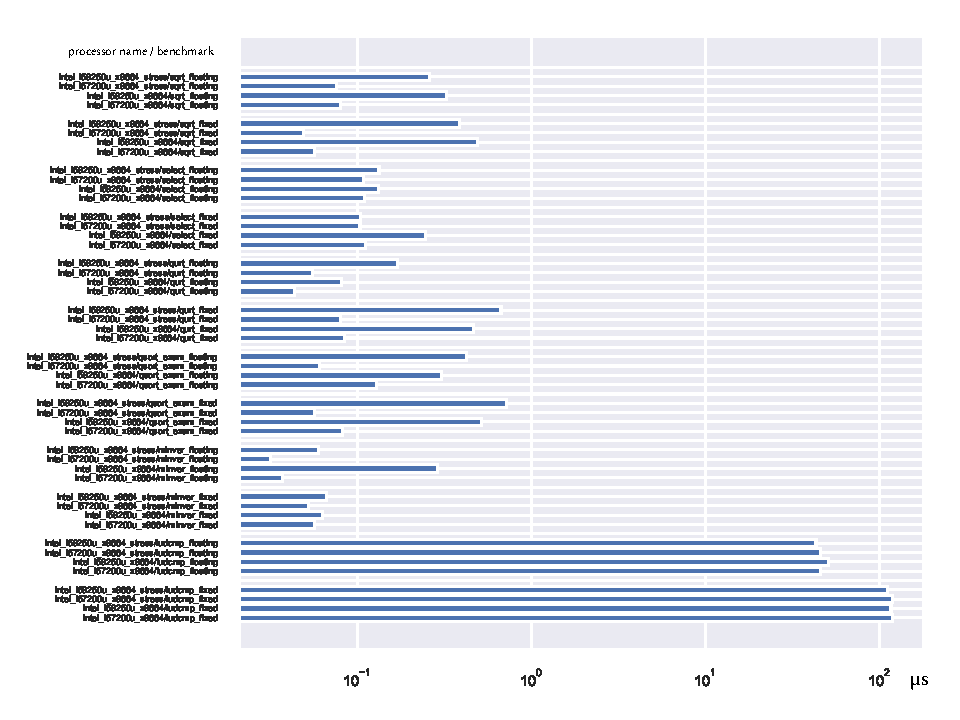
\includegraphics[width=570pt]{intel_histogram.pdf}
\clearpage
In the previous histogram we can identify the following singularities:
Comparing fixed point vs floating point operations:
\begin{itemize}
		\item In the benchmarks \textit{select}, \textit{qurt}, \textit{ludcmp} fixed point operations have a larger standard deviation.
		\item In the benchmarks \textit{sqrt}, \textit{qsort\_exam}, \textit{minver} we observe conflicting behaviours between the two processors (ex: in the \textit{qsort\_exam} benchmark the Intel i5 7200U has a lower standard deviation for the fixed point benchamark with respect to the floating point one. Instead the Intel i5 8250U has the opposite behaviour).
\end{itemize}
Comparing fixed point vs floating point operations with stress:
\begin{itemize}
		\item In the benchmarks \textit{qurt}, \textit{minver}, \textit{ludcmp} fixed point operations have a larger standard deviation.
		\item In the benchmark \textit{select} fixed point operations have a smaller standard deviation.
		\item In the benchmarks \textit{sqrt}, \textit{qsort\_exam} we observe conflicting behaviours between the two processors.
\end{itemize}

\clearpage
\textbf{Smartphones ARMv8a histogram}\newline
\hspace*{-3.2cm}
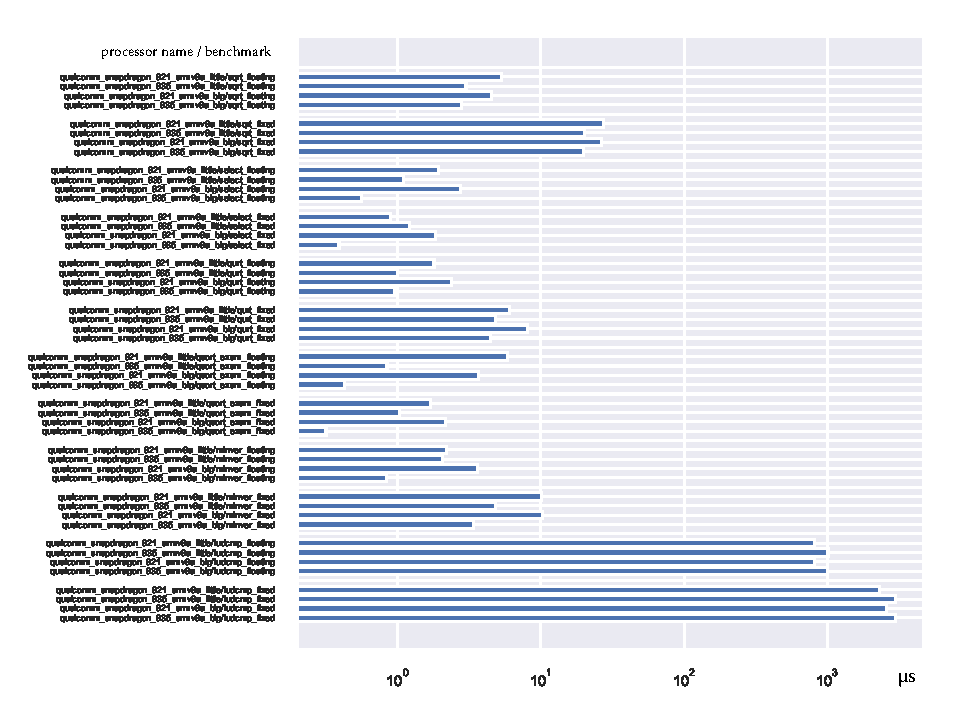
\includegraphics[width=570pt]{smartphones_histogram.pdf}
\clearpage
In the previous histogram we can identify the following singularities:
Comparing fixed point vs floating point operations on the big cluster:
\begin{itemize}
		\item In the benchmarks \textit{sqrt}, \textit{qurt}, \textit{minver}, \textit{ludcmp} fixed point operations have a larger standard deviation.
		\item In the benchmarks \textit{select}, \textit{qsort\_exam} fixed point operations have a smaller standard deviation.
\end{itemize}
Comparing fixed point vs floating point operations on the LITTLE cluster:
\begin{itemize}
		\item In the benchmarks \textit{sqrt}, \textit{qurt}, \textit{minver}, \textit{ludcmp} fixed point operations have a larger standard deviation.
		\item In the benchmarks \textit{select}, \textit{qsort\_exam} we observe conflicting behaviours between the two processors.
\end{itemize}

\clearpage
\textbf{Freescale IMX6 and Odroid XU3 histogram}\newline
\hspace*{-3.2cm}
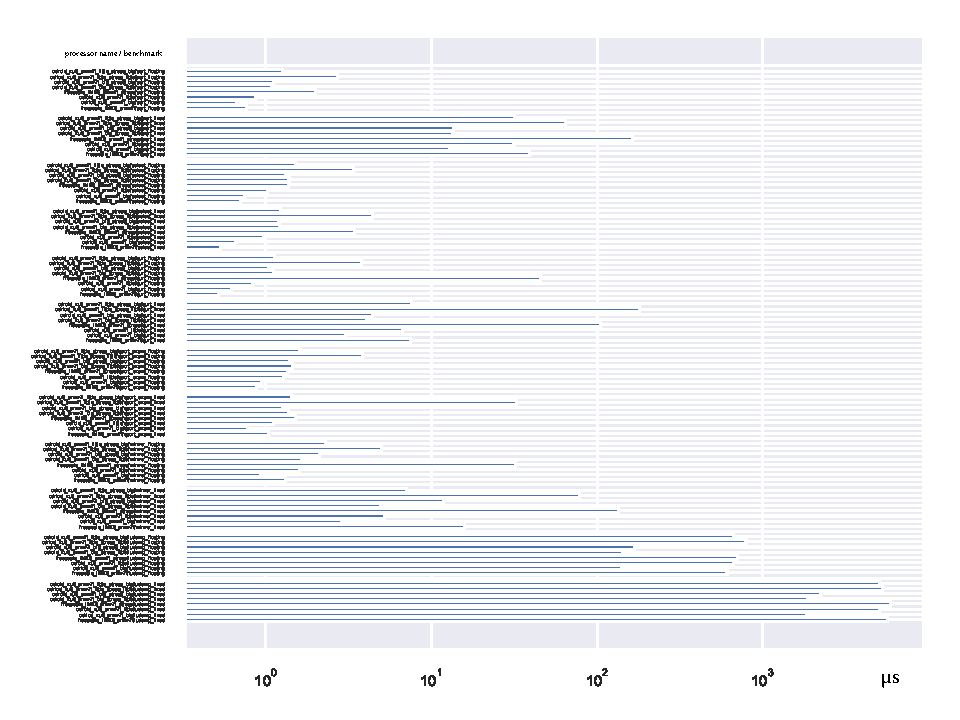
\includegraphics[width=570pt]{boards_histogram.pdf}
\clearpage
In the previous histogram we can identify the following singularities:
Comparing fixed point vs floating point operations on the Freescale IMX6 and the Odroid XU3 big and LITTLE cluster:
\begin{itemize}
		\item In the benchmarks \textit{sqrt}, \textit{qurt}, \textit{minver}, \textit{ludcmp} fixed point operations have a larger standard deviation.
		\item In the benchmark \textit{select} fixed point operations have a smaller standard deviation.
		\item In the benchmark \textit{qsort\_exam} we observe conflicting behaviours between the two processors (Odroid XU3 has lower standard deviation for fixed point operations, Freescale IMX6 has an higher standard deviation).
\end{itemize}
Comparing fixed point vs floating point operations with stress on the Freescale IMX6 and the Odroid XU3 big and LITTLE cluster:
\begin{itemize}
		\item In the benchmarks \textit{sqrt}, \textit{qurt}, \textit{minver}, \textit{ludcmp} fixed point operations have a larger standard deviation.
		\item In the benchmarks \textit{select}, \textit{qsort\_exam} we observe conflicting behaviours between the two processors (In the \textit{select} benchmark the Odroid XU3 running on the LITTLE cluster and stressed on this cluster has a higher standard deviation, the same for the Freescale IMX6 under stress. The exact same behaviour is observed with the benchmark \textit{qsort\_exam}).
\end{itemize}

\section{Conclusions}

\end{document} to your LaTeX file where you want your
% title page.
%
%%%%%%%%%%%%%%%%%%%%%%%%%%%%%%%%%%%%%%%%%
%\title{Title page with logo}
%----------------------------------------------------------------------------------------
%	PACKAGES AND OTHER DOCUMENT CONFIGURATIONS
%----------------------------------------------------------------------------------------

\documentclass[12pt]{article}
\usepackage[english]{babel}
\usepackage[utf8x]{inputenc}
\usepackage{amsmath}
\usepackage{graphicx}
\usepackage{listings}
\usepackage{color}
\usepackage{xcolor}
\usepackage{amssymb}
\usepackage{hyperref}
\usepackage{pdfpages}


\definecolor{dkgreen}{rgb}{0,0.6,0}
\definecolor{gray}{rgb}{0.5,0.5,0.5}
\definecolor{mauve}{rgb}{0.58,0,0.82}

\lstset{frame=tb,
	language=C,
	aboveskip=3mm,
	belowskip=3mm,
	showstringspaces=false,
	columns=flexible,
	basicstyle={\small\ttfamily},
	numbers=none,
	numberstyle=\tiny\color{gray},
	keywordstyle=\color{blue},
	commentstyle=\color{dkgreen},
	stringstyle=\color{mauve},
	breaklines=true,
	breakatwhitespace=true,
	tabsize=3
}

\makeatletter
\newsavebox\myboxA
\newsavebox\myboxB
\newlength\mylenA

\newcommand*\xoverline[2][0.75]{%
	\sbox{\myboxA}{$\m@th#2$}%
	\setbox\myboxB\null% Phantom box
	\ht\myboxB=\ht\myboxA%
	\dp\myboxB=\dp\myboxA%
	\wd\myboxB=#1\wd\myboxA% Scale phantom
	\sbox\myboxB{$\m@th\overline{\copy\myboxB}$}%  Overlined phantom
	\setlength\mylenA{\the\wd\myboxA}%   calc width diff
	\addtolength\mylenA{-\the\wd\myboxB}%
	\ifdim\wd\myboxB<\wd\myboxA%
	\rlap{\hskip 0.5\mylenA\usebox\myboxB}{\usebox\myboxA}%
	\else
	\hskip -0.5\mylenA\rlap{\usebox\myboxA}{\hskip 0.5\mylenA\usebox\myboxB}%
	\fi}
\makeatother

\begin{document}

\begin{titlepage}

\newcommand{\HRule}{\rule{\linewidth}{0.5mm}} % Defines a new command for the horizontal lines, change thickness here

\center % Center everything on the page
 
%----------------------------------------------------------------------------------------
%	HEADING SECTIONS
%----------------------------------------------------------------------------------------

\textsc{\LARGE Politecnico di Milano}\\[1.5cm] % Name of your university/college
\textsc{\Large Dipartimento di Elettronica, Informazione e Bioingegneria}\\[0.5cm] % Major heading such as course name
\textsc{\large HEAPLab Project Report}\\[0.5cm] % Minor heading such as course title

%----------------------------------------------------------------------------------------
%	TITLE SECTION
%----------------------------------------------------------------------------------------

\HRule \\[0.4cm]
{ \huge \bfseries Floating Point Predictability}\\[0.4cm] % Title of your document
\HRule \\[1.5cm]
 
%----------------------------------------------------------------------------------------
%	AUTHOR SECTION
%----------------------------------------------------------------------------------------

\begin{minipage}{0.4\textwidth}
\begin{flushleft} \large
\emph{Authors:}\\
Alessio \textsc{Cantina}\\ % Your name
Simone \textsc{Crippa}
\end{flushleft}
\end{minipage}
~
\begin{minipage}{0.5\textwidth}
\begin{flushright} \large
\emph{Supervisor:} \\
Dr. Federico \textsc{Reghenzani} % Supervisor's Name
\end{flushright}
\end{minipage}\\[1cm]

% If you don't want a supervisor, uncomment the two lines below and remove the section above
%\Large \emph{Author:}\\
%John \textsc{Smith}\\[3cm] % Your name

%----------------------------------------------------------------------------------------
%	DATE SECTION
%----------------------------------------------------------------------------------------

{\large \today}\\[2cm] % Date, change the \today to a set date if you want to be precise

%----------------------------------------------------------------------------------------
%	LOGO SECTION
%----------------------------------------------------------------------------------------


\includegraphics[width=100pt]{heaplogo.pdf}\\[1cm] % Include a department/university logo - this will require the graphicx package
 
%----------------------------------------------------------------------------------------

\vfill % Fill the rest of the page with whitespace

\end{titlepage}




\begin{abstract}
\textcolor{red}{Your abstract. - Summarize your work.}

This project aims to investigate floating point vs fixed point predictability.

To achieve this result, we have used 6 Worst Case Execution Time (WCET) benchmarks which involve a large number of floating point instructions.
We converted these benchmarks using only fixed point variables and then we added the logic to obtain multiple measurements.

Finally, we computed and analysed 8 statistics to find out if floating point operations or fixed point operations are more predictable.

\end{abstract}

\section{Introduction}

\textcolor{red}{Your introduction goes here! Some examples of commonly used commands and features are listed below, to help you get started.}

In this section we describe the devices used for the benchmarks and all the commands used to process the benchmarks.

\subsection{Devices used}

To have a better view of the problem, we decided to get samples from devices with different architecture.
In this project, we considered 3 architectures and 6 devices.\newline 
armv7l devices:
\begin{itemize}
	\item Device name: Freescale i.MX 6 Quad. Processor configuration: 4x Cortex-A9 @ 1.2 GHz
	\item Device name: ODROID-XU3. Processor name: Exynos 5422. Processor configuration: big.LITTLE 8 cores, 4x Cortex-A15 @ 2.0 GHz, 4x Cortex-A7 @ 1.4 GHz 
\end{itemize}
armv8a devices:
\begin{itemize}
	\item Device name: Xiaomi Mi 5s. Processor name: Snapdragon 821 (MSM8996). Processor configuration: big.LITTLE 4 cores: 2x Kryo @ 2.15 GHz, 2x Kryo @ 1.6 GHz
	\item Device name: Xiaomi Mi Mix 2. Processor name: Snapdragon 835 (MSM8998). Processor configuration: big.LITTLE 8 cores: 4x Kryo @ 2.45 GHz, 4x Kryo @ 1.9 GHz
\end{itemize}
x86\_64 devices:
\begin{itemize}
	\item Device name: Dell XPS 13 9360. Processor name: Intel i5 8250U. Processor configuration: 4 cores (8 threads) @ 3.40 GHz
	\item Device name: Dell Vostro 15 3568. Processor name: Intel i5 7200U.
	Processor configuration: 2 cores (4 threads) @ 3.10 GHz
\end{itemize}
\subsection{Compiling commands}

\begin{itemize}
	\item Compile a floating point benchmark: \begin{verbatim}gcc -o "output_name" "benchmark_name"\end{verbatim}
	\item Cross-compile a benchmark, useful to execute a benchmark on a smartphone with ARM processor: \begin{verbatim}arm-linux-gnueabi-gcc -static -march="arm_platform" -o 
	"output_name" "benchmark_name"\end{verbatim}
	\item To compile a fixed point benchmark remember to append at the end of the command the library used for fixed point operations: \begin{verbatim}fixed_op_64bit.c\end{verbatim}
\end{itemize}


\subsection{make commands}

A makefile has been produced so that make can be used to compile and execute all the benchmarks at once:

\begin{itemize}
	\item Initialize the project directory with support folders:\begin{verbatim}make init\end{verbatim}
	\item Compile all the benchmarks: \begin{verbatim}make\end{verbatim}
	\item Execute all the benchmarks: \begin{verbatim}make run\end{verbatim}
	\item Clear the project directory: \begin{verbatim}make clean\end{verbatim}
\end{itemize}

Note: the makefile supports gcc compilation as is, but it needs to be modified for cross compilation. Detailed instructions are available inside the makefile.

\subsection{Additional commands}

These commands are used to run benchmarks with a stress test running on the CPU cache

\begin{itemize}
	\item Stress the CPU cache on a specific set of CPUs:\begin{verbatim}taskset -c cpu_list stress-ng --cache N \end{verbatim} where cpu\_list is the select cluster (start\_CPU - end\_CPU) and N is the number of worker threads (1 thread for each CPU core)
	\item Execute the benchmarks on a specific set of CPUs: \begin{verbatim}taskset -c cpu_list\end{verbatim}
\end{itemize}

\section{Design and Implementation}

\subsection{Benchmarks}

To investigate this issue, we selected 6 floating point benchmarks from \href{http://www.mrtc.mdh.se/projects/wcet/benchmarks.html}{mrtc.mdh.se}.
These are the selected benchmarks:
\begin{enumerate}
	\item \textbf{ludcmp}: implementation of the \href{https://en.wikipedia.org/wiki/LU_decomposition}{LU decomposition} algorithm
	\item \textbf{minve}r: inversion of a floating point matrix
	\item \textbf{qsort\_exam}: non-recursive implementation of quick sort algorithm
	\item \textbf{qurt}: root computation of quadratic equations
	\item \textbf{select}: function to select the ${N}^{th}$ largest number in a floating point array
	\item \textbf{sqrt}: square root function implemented by Taylor series
\end{enumerate}

Since there is no automatic way in C to convert floating point operations into fixed point, we have defined rules to convert floating point benchmarks into fixed points.
\begin{enumerate}
	\item Convert all the floating values into fixed point values in a fair way, keeping the same variable dimension:
	\begin{itemize}
		\item float $\rightarrow$ int32\_t	
		\item double $\rightarrow$ int64\_t
	\end{itemize}
	\item Multiply every floating point value by ${2}^{SHIFT\_AMOUNT}$, where SHIFT\_AMOUNT defines the precision of the fixed point values.
	\item Convert every multiplication and division into the corresponding fixed point function:
	\begin{itemize}
		\item multiplication $\rightarrow$ fixed\_mul\_64bit	
		\item division $\rightarrow$ fixed\_div\_64bit
	\end{itemize}
\end{enumerate}

Moreover, all benchmarks are executed on random generated numbers, except qurt which computes multiple times the inversion of a matrix.\newline
Note: random numbers are generated setting a common seed using the \textit{srand()} function, so that every benchmark in its floating and fixed version works on the same values.
\subsection{Sampling of the benchmarks}

Original benchmarks have no built-in method to obtain the elapsed execution time. We have implemented and integrated in C a function which randomly generates arguments for the benchmark and measures the elapsed time.
Measurements are stored in text files for future analysis.

This is an example of the main function:
\begin{itemize}
	\item srand() is used to generate random numbers, using a seed to keep track of generated numbers.
	\item EXEC\_NUM is a constant which regulates the number of samples generated. In our case, we generate 100.000 samples.
	\item function\_to\_call(val) is the benchmark function with the argument.
	\item diff(timespec,timespec) is a support function which makes the difference between two time instants.
	\item CLOCK\_MONOTONIC\_RAW is used to get the time instant from the system without alterations (even from ntp)
	\item SHIFT\_AMOUNT is used to convert floating point values into fixed points, an higher SHIFT\_AMOUNT means an higher decimal precision.
\end{itemize}
\begin{lstlisting}
int main()
{
	struct timespec start,end;
	FILE * fp;
	fp = fopen ("benchmark_results.txt","w");
	int64_t val;
	srand(5);
	for (int i=0; i< EXEC_NUM ; i++){
		//convert float to int64 only if the benchmark is fixed point, if not no conversion is done
		val = (int64_t)((((rand() % 10000) / 100) - 50) * pow(2,SHIFT_AMOUNT));
		
		clock_gettime(CLOCK_MONOTONIC_RAW, &start);
		function_to_call(val);
		clock_gettime(CLOCK_MONOTONIC_RAW, &end);
		
		fprintf (fp, "%lld\n",(long long)(diff(start,end).tv_sec * pow(10,9))+(long long)diff(start,end).tv_nsec);
	}
	
	fclose (fp);
	return 0;
}
\end{lstlisting}

\subsection{Fixed point operations}

To support fixed point operations we had to introduce a shift amount, so that floating point numbers can be represented as integers with a fixed precision, given by the shift amount.\newline
Since we have analysed different architectures we had to take into account the limitations of the selected architectures.
x86\_64 have the support for 128-bit variables, which are necessary to compute multiplications and divisions. Instead, ARM architectures have no support for 128-bit variables, so we implemented a support library to handle this discrepancy.
The library automatically select the operations by checking if the architecture support 128-bit integers, if there is no support, the benchmark will use a portable implementation of multiplication and division which are based on 64-bit integers.\newline
Our implementation of fixed division and multiplication works with a variable shift amount, in our benchmarks we have always used a shift amount of 30 because in our scenario it allows to have the necessary precision.\newline
Note: to guarantee fairness we use hard-coded values for constants in benchmarks that are shifted by 30-bits, even though operations supports dynamical shift amounts these values have to be modified to comply with the new selected shift amount.\newline

\textbf{fixed\_div for 128-bit support}

\begin{lstlisting}
int64_t fixed_div_64(int64_t x, int64_t y, int shift_amount)
{
    return ((((__int128)x << shift_amount) / y));
}
\end{lstlisting}

\textbf{fixed\_mul for 128-bit support}

\begin{lstlisting}
int64_t fixed_mul_64(int64_t x, int64_t y, int shift_amount)
{
	return (int64_t)((((__int128)x * (__int128)y)) >> shift_amount);
}
\end{lstlisting}

\textbf{fixed\_div without 128-bit support}\newline
To implement the divison mantaining the 128 bit precision needed during the divison operation,  the dividend is splitted into two 64 bit integers. Then the divison is perfomed using the technique that can be found at this \href{https://codereview.stackexchange.com/questions/67962/mostly-portable-128-by-64-bit-division}{link}.\newline

\textbf{fixed\_mul without 128-bit support}\newline
To implement the multiplication mantaining the 128 bit precision needed during the multiplication operation,  the two factors are splitted into two 64 bit integers each. Then the multiplication is perfomed using the technique that can be found at this \href{https://stackoverflow.com/questions/31652875/fastest-way-to-multiply-two-64-bit-ints-to-128-bit-then-to-64-bit}{link}.



\subsection{Statistics used}
To compare floating point results to fixed point results we computed through a Python script 8 metrics useful to analyse the predictability of a benchmark.

\begin{enumerate}
	\item Minimum execution time, computed through the Python built-in function \textit{min()}
	\item Maximum execution time, computed through the Python built-in function \textit{max()}
	\item Sample mean, computed through the Python module numpy as \textit{numpy.mean()}, the formula is: $$\xoverline[0.8]{x} = \frac{X_1 + X_2 + \cdots + X_n}{n}
	= \frac{1}{n}\sum_{i}^{n} X_i$$
	\item Sample variance, computed through the Python module numpy as \textit{numpy.var()}, the formula is:$${s}^{2} = \frac{\sqrt{\sum_{i}^{n} {(x_i - \xoverline[0.8]{x})}^{2}}}{n-1}$$
	\item Sample standard deviation, computed through the Python module statistics as \textit{statistics.stdev()}, the formula is:
	$$s = \frac{\sqrt{\sum_{i}^{n} (x_i - \xoverline[0.8]{x})}}{n-1}$$
	\item KPSS test statistic, computed through the Python module statsmodels as \textit{statsmodels.tsa.stattools.kpss()}, the formula is:$$S = \frac{{T}^{-2}\sum_{t=1}^{T} {\hat{S}_t}^{2}}{\sigma_\epsilon}$$
	Where:
	\begin{itemize}
		\item T is the sample size
		\item ${\sigma_\epsilon}$ is the long-run variance
		\item ${\hat{S}_t} = \sum_{i}^{t}e(t)$ is the partial sum of the errors of the regression $y(t)$
	\end{itemize}
	\item BDS test statistic, computed through the Python module statsmodels as \textit{statsmodels.tsa.stattools.bds()}, the formula is: $$BDS_{\epsilon,m} = \frac{\sqrt{N}[C_{\epsilon,m}-{(C_{\epsilon,1})}^{m}]}{\sqrt{V_{\epsilon,m}}}$$
	Where:
	\begin{itemize}
		\item $C_{\epsilon,m} = \frac{1}{N_m(N_m-1)}\sum_{i\not=j}{I_{i,j;\epsilon}}$\\[0.1cm]
		Where:
		\begin{itemize}
			\item m is the number of embedding dimensions, used to embed the time series into m-dimensional vectors.
			\item ${I_{i,j;\epsilon}} = 1 \;\; if ||{x}^{m}_i - {x}^{m}_j|| <= \epsilon  \;\; = 0 \;\; otherwise$
		\end{itemize}
		
		\item $V_{\epsilon,m} = 4[{K}^{m} + 2\sum_{j=1}^{m-1}{K}^{m-j}{C}^{2j}_\epsilon + {(m-1)}^{2}{C}^{2m}_\epsilon - {m}^{2}K{C}^{2m-2}_\epsilon]$
		Where:
		\begin{itemize}
			\item $K=K_\epsilon = \frac{6}{N_m(N_m-1)*(N_m-2)}\sum_{i<j<N}h_{i,j,N;\epsilon}$
			\item $h_{i,j,N;\epsilon} = \frac{[I_{i,j;\epsilon}I_{j,N;\epsilon}+I_{i,N;\epsilon}I_{N,j;\epsilon}+I_{j,i;\epsilon}I_{i,N;\epsilon}]}{3}$
		\end{itemize}
	\end{itemize}
	We know under some hypothesis, that the quantity $[C_{\epsilon,m}-{(C_{\epsilon,1})}^{m}]$ can be considered as an asymptotic normal distribution with zero mean and variance $V_{\epsilon,m}$
	\item Hurst exponent, computed through the Python module hurst as \textit{compute\_Hc(array, kind='change', simplified=True)}, the formula is:\newline
	$\operatorname{E} \left [ \frac{R(n)}{S(n)} \right ]=C n^H  \text{  as } n \to \infty  \, $
	\newline Where:
	\begin{itemize}
		\item $R(n)$ is the range of the first n cumulative deviations from the mean, and $s(n)$ is their standard deviation
		\item $\operatorname{E} \left [x \right ] \,$ is the expected value
		\item n is the time span of the observation (number of data points in a time series)
		\item C is a constant.
	\end{itemize}
\end{enumerate}

We are interested in execution time predictability, so we need to compare how much the measurements are spread through sample standard deviation and sample variance.
\href{http://debis.deu.edu.tr/userweb//onder.hanedar/dosyalar/kpss.pdf}{KPSS} test statistic is a one tailed test, which indicates if the time series is stationary around a mean or a linear trend. A stationary time series have constant statistical properties (like mean and variance) over time.
\begin{itemize}
	\item Null hypothesis: the data is stationary
	\item Alternative hypothesis: the data is not stationary
\end{itemize}
Instead, \href{https://www.researchgate.net/publication/46554708_A_Fast_Algorithm_for_the_BDS_Statistic}{BDS} statistic is a double tailed test, which indicates if the time series is serial dependent.
\begin{itemize}
 	\item Null hypothesis: the data is independently and identically distributed (I.I.D.)
 	\item Alternative hypothesis: the data is not I.I.D.
\end{itemize}

Since BDS test statistic complexity increase with the sample size, it can't be done on all the samples at once, instead we compute it using a sliding window on the samples and then select the maximum BDS obtained.\newline
Hurst Exponent is used to measure the long-term memory of a time series:
\begin{enumerate}
	\item If the Hurst Exponent is in the 0.5-1 range, we have a time series with long-term positive autocorrelation, meaning that an high value in the series will be followed by another high value and also the future values will tend to be high.
	\item If the Hurst Exponent is in the 0-0.5 range, we have a time series with long-term switching between high and low values so a single high value will probably be followed by a low value and also the future values will keep this tendency to switch between high and low values.
	\item If the Hurst Exponent is equal to 0.5, we have 2 different scenarios:
	\begin{itemize}
		\item A completely uncorrelated series
		\item A time series with alternating positive and negative autocorrelation but the absolute values of the autocorrelation decay exponentially to zero.
	\end{itemize}
\end{enumerate}



\section{Experimental Results}
Now a series of histrograms are displayed to better comprehend the behaviour of the different architectures.
These histrograms show the standard deviation expressed in microseconds for each benchmark and each processor.
Note: that the x scale is logaritmic.\newline

\textbf{Intel x86\_64 histogram}\newline
\hspace*{-3.2cm}
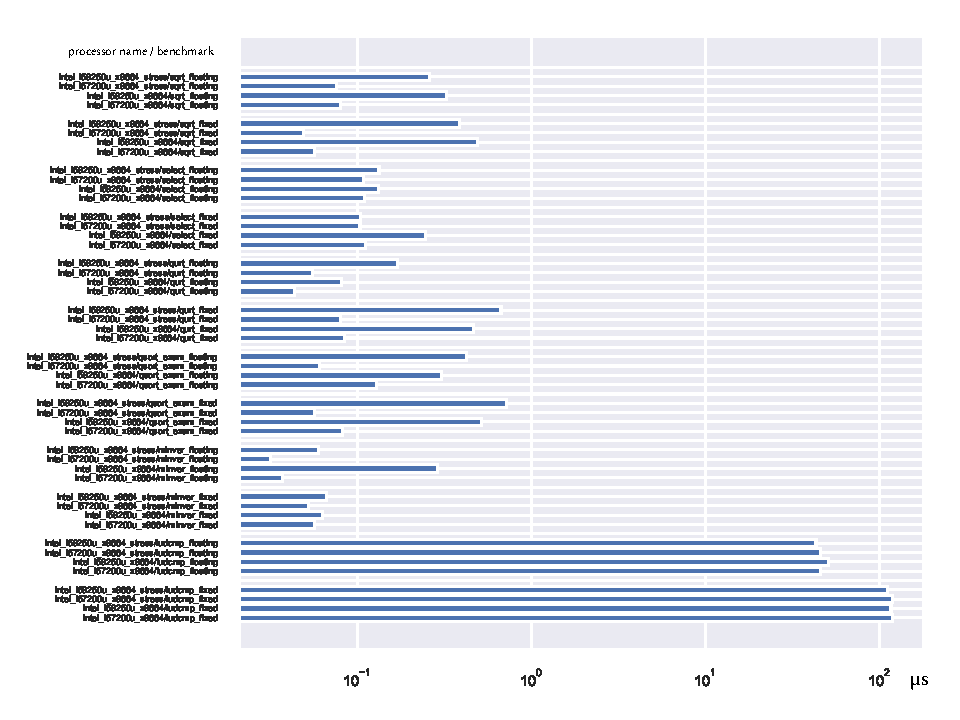
\includegraphics[width=570pt]{intel_histogram.pdf}
\clearpage
In the previous histogram we can identify the following singularities:
Comparing fixed point vs floating point operations:
\begin{itemize}
		\item In the benchmarks \textit{select}, \textit{qurt}, \textit{ludcmp} fixed point operations have a larger standard deviation.
		\item In the benchmarks \textit{sqrt}, \textit{qsort\_exam}, \textit{minver} we observe conflicting behaviours between the two processors (ex: in the \textit{qsort\_exam} benchmark the Intel i5 7200U has a lower standard deviation for the fixed point benchamark with respect to the floating point one. Instead the Intel i5 8250U has the opposite behaviour).
\end{itemize}
Comparing fixed point vs floating point operations with stress:
\begin{itemize}
		\item In the benchmarks \textit{qurt}, \textit{minver}, \textit{ludcmp} fixed point operations have a larger standard deviation.
		\item In the benchmark \textit{select} fixed point operations have a smaller standard deviation.
		\item In the benchmarks \textit{sqrt}, \textit{qsort\_exam} we observe conflicting behaviours between the two processors.
\end{itemize}

\clearpage
\textbf{Smartphones ARMv8a histogram}\newline
\hspace*{-3.2cm}
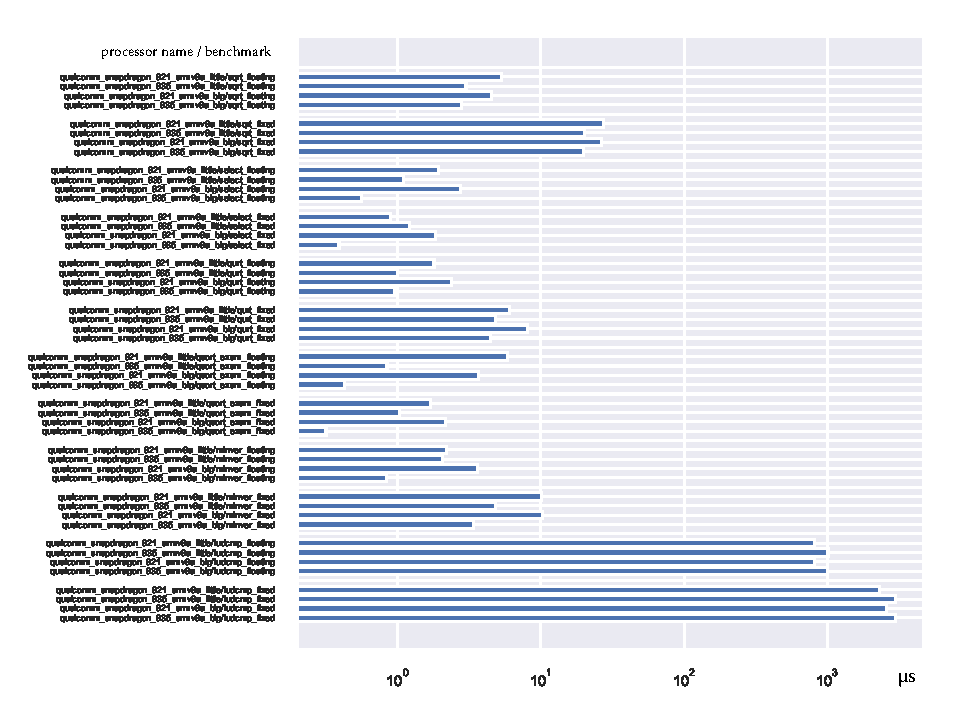
\includegraphics[width=570pt]{smartphones_histogram.pdf}
\clearpage
In the previous histogram we can identify the following singularities:
Comparing fixed point vs floating point operations on the big cluster:
\begin{itemize}
		\item In the benchmarks \textit{sqrt}, \textit{qurt}, \textit{minver}, \textit{ludcmp} fixed point operations have a larger standard deviation.
		\item In the benchmarks \textit{select}, \textit{qsort\_exam} fixed point operations have a smaller standard deviation.
\end{itemize}
Comparing fixed point vs floating point operations on the LITTLE cluster:
\begin{itemize}
		\item In the benchmarks \textit{sqrt}, \textit{qurt}, \textit{minver}, \textit{ludcmp} fixed point operations have a larger standard deviation.
		\item In the benchmarks \textit{select}, \textit{qsort\_exam} we observe conflicting behaviours between the two processors.
\end{itemize}

\clearpage
\textbf{Freescale IMX6 and Odroid XU3 histogram}\newline
\hspace*{-3.2cm}
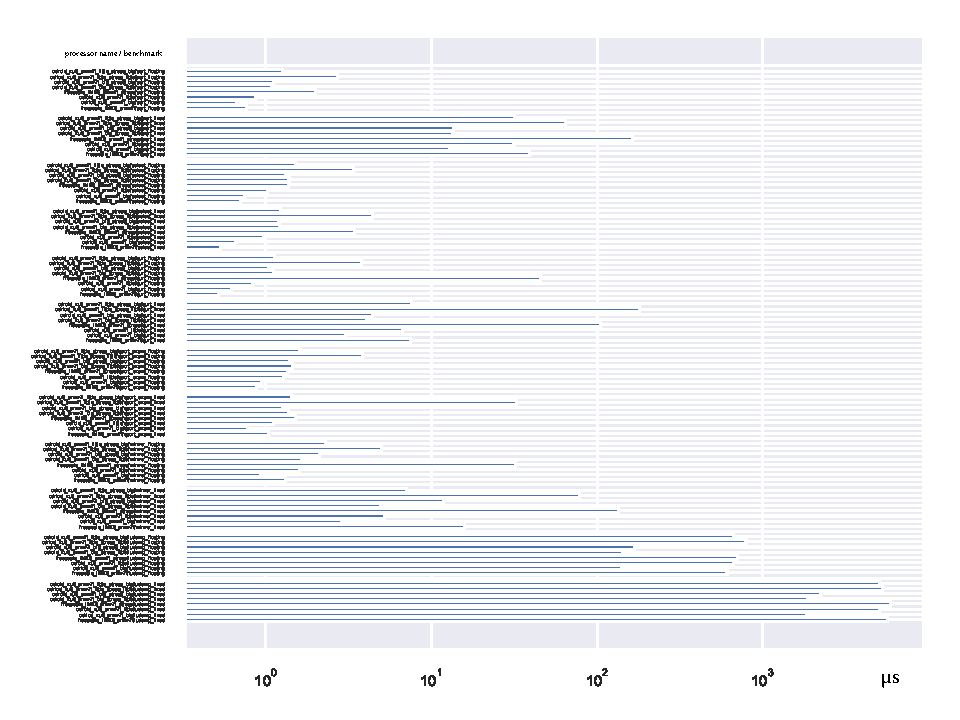
\includegraphics[width=570pt]{boards_histogram.pdf}
\clearpage
In the previous histogram we can identify the following singularities:
Comparing fixed point vs floating point operations on the Freescale IMX6 and the Odroid XU3 big and LITTLE cluster:
\begin{itemize}
		\item In the benchmarks \textit{sqrt}, \textit{qurt}, \textit{minver}, \textit{ludcmp} fixed point operations have a larger standard deviation.
		\item In the benchmark \textit{select} fixed point operations have a smaller standard deviation.
		\item In the benchmark \textit{qsort\_exam} we observe conflicting behaviours between the two processors (Odroid XU3 has lower standard deviation for fixed point operations, Freescale IMX6 has an higher standard deviation).
\end{itemize}
Comparing fixed point vs floating point operations with stress on the Freescale IMX6 and the Odroid XU3 big and LITTLE cluster:
\begin{itemize}
		\item In the benchmarks \textit{sqrt}, \textit{qurt}, \textit{minver}, \textit{ludcmp} fixed point operations have a larger standard deviation.
		\item In the benchmarks \textit{select}, \textit{qsort\_exam} we observe conflicting behaviours between the two processors (In the \textit{select} benchmark the Odroid XU3 running on the LITTLE cluster and stressed on this cluster has a higher standard deviation, the same for the Freescale IMX6 under stress. The exact same behaviour is observed with the benchmark \textit{qsort\_exam}).
\end{itemize}

\section{Conclusions}

\end{document} to your LaTeX file where you want your
% title page.
%
%%%%%%%%%%%%%%%%%%%%%%%%%%%%%%%%%%%%%%%%%
%\title{Title page with logo}
%----------------------------------------------------------------------------------------
%	PACKAGES AND OTHER DOCUMENT CONFIGURATIONS
%----------------------------------------------------------------------------------------

\documentclass[12pt]{article}
\usepackage[english]{babel}
\usepackage[utf8x]{inputenc}
\usepackage{amsmath}
\usepackage{graphicx}
\usepackage{listings}
\usepackage{color}
\usepackage{xcolor}
\usepackage{amssymb}
\usepackage{hyperref}
\usepackage{pdfpages}


\definecolor{dkgreen}{rgb}{0,0.6,0}
\definecolor{gray}{rgb}{0.5,0.5,0.5}
\definecolor{mauve}{rgb}{0.58,0,0.82}

\lstset{frame=tb,
	language=C,
	aboveskip=3mm,
	belowskip=3mm,
	showstringspaces=false,
	columns=flexible,
	basicstyle={\small\ttfamily},
	numbers=none,
	numberstyle=\tiny\color{gray},
	keywordstyle=\color{blue},
	commentstyle=\color{dkgreen},
	stringstyle=\color{mauve},
	breaklines=true,
	breakatwhitespace=true,
	tabsize=3
}

\makeatletter
\newsavebox\myboxA
\newsavebox\myboxB
\newlength\mylenA

\newcommand*\xoverline[2][0.75]{%
	\sbox{\myboxA}{$\m@th#2$}%
	\setbox\myboxB\null% Phantom box
	\ht\myboxB=\ht\myboxA%
	\dp\myboxB=\dp\myboxA%
	\wd\myboxB=#1\wd\myboxA% Scale phantom
	\sbox\myboxB{$\m@th\overline{\copy\myboxB}$}%  Overlined phantom
	\setlength\mylenA{\the\wd\myboxA}%   calc width diff
	\addtolength\mylenA{-\the\wd\myboxB}%
	\ifdim\wd\myboxB<\wd\myboxA%
	\rlap{\hskip 0.5\mylenA\usebox\myboxB}{\usebox\myboxA}%
	\else
	\hskip -0.5\mylenA\rlap{\usebox\myboxA}{\hskip 0.5\mylenA\usebox\myboxB}%
	\fi}
\makeatother

\begin{document}

\begin{titlepage}

\newcommand{\HRule}{\rule{\linewidth}{0.5mm}} % Defines a new command for the horizontal lines, change thickness here

\center % Center everything on the page
 
%----------------------------------------------------------------------------------------
%	HEADING SECTIONS
%----------------------------------------------------------------------------------------

\textsc{\LARGE Politecnico di Milano}\\[1.5cm] % Name of your university/college
\textsc{\Large Dipartimento di Elettronica, Informazione e Bioingegneria}\\[0.5cm] % Major heading such as course name
\textsc{\large HEAPLab Project Report}\\[0.5cm] % Minor heading such as course title

%----------------------------------------------------------------------------------------
%	TITLE SECTION
%----------------------------------------------------------------------------------------

\HRule \\[0.4cm]
{ \huge \bfseries Floating Point Predictability}\\[0.4cm] % Title of your document
\HRule \\[1.5cm]
 
%----------------------------------------------------------------------------------------
%	AUTHOR SECTION
%----------------------------------------------------------------------------------------

\begin{minipage}{0.4\textwidth}
\begin{flushleft} \large
\emph{Authors:}\\
Alessio \textsc{Cantina}\\ % Your name
Simone \textsc{Crippa}
\end{flushleft}
\end{minipage}
~
\begin{minipage}{0.5\textwidth}
\begin{flushright} \large
\emph{Supervisor:} \\
Dr. Federico \textsc{Reghenzani} % Supervisor's Name
\end{flushright}
\end{minipage}\\[1cm]

% If you don't want a supervisor, uncomment the two lines below and remove the section above
%\Large \emph{Author:}\\
%John \textsc{Smith}\\[3cm] % Your name

%----------------------------------------------------------------------------------------
%	DATE SECTION
%----------------------------------------------------------------------------------------

{\large \today}\\[2cm] % Date, change the \today to a set date if you want to be precise

%----------------------------------------------------------------------------------------
%	LOGO SECTION
%----------------------------------------------------------------------------------------


\includegraphics[width=100pt]{heaplogo.pdf}\\[1cm] % Include a department/university logo - this will require the graphicx package
 
%----------------------------------------------------------------------------------------

\vfill % Fill the rest of the page with whitespace

\end{titlepage}




\begin{abstract}

This project aims to investigate floating point vs fixed point predictability.

To achieve this result, we have used six Worst Case Execution Time (WCET) benchmarks which involve a large number of floating point instructions.
We converted these benchmarks using only fixed point variables and then we added the logic to obtain multiple measurements. To obtain a general overview of the problem, these benchmarks were executed on different devices with different architectures and where it was possible with a perturbation, obtaining distinct time-series in all the possible conditions.

Finally, we computed and analysed eight statistics to find out if floating point operations or fixed point operations are more predictable, by comparing them through histograms and statistics tests.
\clearpage
\end{abstract}

\section{Introduction}

In this section we describe the devices used for the benchmarks and all the commands used to process the benchmarks.

\subsection{Devices used}

To have a better view of the problem, we decided to get samples from devices with different architecture.
In this project, we considered 3 architectures and 6 devices.\newline 
\textbf{armv7l devices}:
\begin{itemize}
	\item Device name: Freescale i.MX 6 Quad\newline Processor configuration: 4x Cortex-A9 @ 1.2 GHz
	\item Device name: ODROID-XU3 \newline Processor name: Exynos 5422\newline Processor configuration: big.LITTLE 8 cores, 4x Cortex-A15 @ 2.0 GHz, 4x Cortex-A7 @ 1.4 GHz 
\end{itemize}
\textbf{armv8a devices}:
\begin{itemize}
	\item Device name: Xiaomi Mi 5s\newline Processor name: Snapdragon 821 (MSM8996) \newline Processor configuration: big.LITTLE 4 cores: 2x Kryo @ 2.15 GHz, 2x Kryo @ 1.6 GHz
	\item Device name: Xiaomi Mi Mix 2\newline Processor name: Snapdragon 835 (MSM8998)\newline Processor configuration: big.LITTLE 8 cores: 4x Kryo @ 2.45 GHz, 4x Kryo @ 1.9 GHz
\end{itemize}
\textbf{x86\_64 devices}:
\begin{itemize}
	\item Device name: Dell XPS 13 9360\newline Processor name: Intel i5 8250U \newline Processor configuration: 4 cores (8 threads) @ 3.40 GHz
	\item Device name: Dell Vostro 15 3568 \newline Processor name: Intel i5 7200U
	\newline Processor configuration: 2 cores (4 threads) @ 3.10 GHz
\end{itemize}
\clearpage
\subsection{Compiling commands}

\begin{itemize}
	\item Compile a floating point benchmark: \begin{verbatim}gcc -o "output_name" "benchmark_name"\end{verbatim}
	\item Cross-compile a benchmark, useful to execute a benchmark on a smartphone with ARM processor: \begin{verbatim}arm-linux-gnueabi-gcc -static -march="arm_platform" -o 
	"output_name" "benchmark_name"\end{verbatim}
	\item To compile a fixed point benchmark remember to append at the end of the command the library used for fixed point operations: \begin{verbatim}fixed_op_64bit.c\end{verbatim}
\end{itemize}


\subsection{make commands}

A makefile has been produced so that make can be used to compile and execute all the benchmarks at once:

\begin{itemize}
	\item Initialize the project directory with support folders:\begin{verbatim}make init\end{verbatim}
	\item Compile all the benchmarks: \begin{verbatim}make\end{verbatim}
	\item Execute all the benchmarks: \begin{verbatim}make run\end{verbatim}
	\item Clear the project directory: \begin{verbatim}make clean\end{verbatim}
\end{itemize}

Note: the makefile supports gcc compilation as is, but it needs to be modified for cross compilation. Detailed instructions are available inside the makefile.

\subsection{Additional commands}

These commands are used to run benchmarks with a stress test running on the CPU cache

\begin{itemize}
	\item Stress the CPU cache on a specific set of CPUs:\begin{verbatim}taskset -c cpu_list stress-ng --cache N \end{verbatim} where cpu\_list is the selected cluster (start\_CPU - end\_CPU) and N is the number of worker threads (1 thread for each CPU core)
	\item Execute the benchmarks on a specific set of CPUs: \begin{verbatim}taskset -c cpu_list "benchmark_to_execute"\end{verbatim}
\end{itemize}
\clearpage
\section{Design and Implementation}

\subsection{Benchmarks}

To investigate this issue, we selected 6 floating point benchmarks from \href{http://www.mrtc.mdh.se/projects/wcet/benchmarks.html}{mrtc.mdh.se}.
These are the selected benchmarks:
\begin{enumerate}
	\item \textbf{ludcmp}: implementation of the \href{https://en.wikipedia.org/wiki/LU_decomposition}{LU decomposition} algorithm
	\item \textbf{minver}: inversion of a floating point matrix
	\item \textbf{qsort\_exam}: non-recursive implementation of quick sort algorithm
	\item \textbf{qurt}: root computation of quadratic equations
	\item \textbf{select}: function to select the ${N}^{th}$ largest number in a floating point array
	\item \textbf{sqrt}: square root function implemented by Taylor series
\end{enumerate}

Since there is no automatic way in C to convert floating point operations into fixed point, we have defined rules to convert floating point benchmarks into fixed points.
\begin{enumerate}
	\item Convert all the floating point values into fixed point values in a fair way, keeping the same variable dimension:
	\begin{itemize}
		\item float $\rightarrow$ int32\_t	
		\item double $\rightarrow$ int64\_t
	\end{itemize}
	\item Multiply every floating point value by ${2}^{SHIFT\_AMOUNT}$, where SHIFT\_AMOUNT defines the precision of the fixed point values.
	\item Convert all the hard-coded constants to their corresponding fixed point value maintaining the same SHIFT\_AMOUNT as before.
	\item Convert every multiplication and division into the corresponding fixed point function:
	\begin{itemize}
		\item multiplication $\rightarrow$ fixed\_mul\_64bit	
		\item division $\rightarrow$ fixed\_div\_64bit
	\end{itemize}
\end{enumerate}

Moreover, all benchmarks are executed on random generated numbers, except qurt which computes multiple times the inversion of a matrix.\newline
Note: random numbers are generated setting a common seed using the \textit{srand()} function, so that every benchmark in its floating and fixed version works on the same input values.
\subsection{Sampling of the benchmarks}

Time samples from the benchmarks are generated by executing the previous benchmarks on the devices indicated in section \textit{Devices used} (1.1) with different configurations:
\begin{itemize}
	\item For big.LITTLE architectures, samples have been generated considering the big cluster and the LITTLE cluster.
	\item For armv7l and x86\_64, samples have been generated also by applying a perturbation on the CPU (more on the that in section 2.4 \textit{Benchmarks perturbation})
\end{itemize}
Original benchmarks have no built-in method to obtain the elapsed execution time. We have implemented and integrated in C a function which randomly generates arguments for the benchmark and measures the elapsed time.
Measurements are stored in text files for future analysis.

This is an example of the main function:
\begin{itemize}
	\item \textit{srand()} is used to generate random numbers, using a seed to generate a predictable series of numbers.
	\item EXEC\_NUM is a constant which regulates the number of samples generated. In our case, we generate 100.000 samples by executing 100.000 times the benchmark.
	\item \textit{function\_to\_call(val)} is the benchmark function with the argument, val is the random generated input.
	\item \textit{diff(timespec,timespec)} is a support function which makes the difference between two time instants.
	\item CLOCK\_MONOTONIC\_RAW is used to get the time instant from the system without alterations (even from ntp).
	\item SHIFT\_AMOUNT is used to convert floating point values into fixed point, an higher SHIFT\_AMOUNT means an higher decimal precision.
\end{itemize}
\begin{lstlisting}
int main()
{
	struct timespec start,end;
	FILE * fp;
	fp = fopen ("benchmark_results.txt","w");
	int64_t val;
	srand(5);
	for (int i=0; i< EXEC_NUM ; i++){
		//convert float to int64 only if the benchmark is fixed point, if not no conversion is done
		val = (int64_t)((((rand() % 10000) / 100) - 50) * pow(2,SHIFT_AMOUNT));
		
		clock_gettime(CLOCK_MONOTONIC_RAW, &start);
		function_to_call(val);
		clock_gettime(CLOCK_MONOTONIC_RAW, &end);
		
		fprintf (fp, "%lld\n",(long long)(diff(start,end).tv_sec * pow(10,9))+(long long)diff(start,end).tv_nsec);
	}
	
	fclose (fp);
	return 0;
}
\end{lstlisting}

\subsection{Fixed point operations}

To support fixed point operations we had to introduce a shift amount, so that floating point numbers can be represented as integers with a fixed precision given by the shift amount.\newline
In the analysed benchmarks all the divisions and multiplications were done between double precision variables, which correspond to \textit{int64\_t} fixed point variables. As a consequence, we built a library \textit{fixed\_op\_64bit.c} which supports only multiplications and divisions between \textit{int64\_t} variables. \newline
Since we have analysed different architectures we had to take into account the limitations of the selected architectures.\newline
x86\_64 has the support for 128-bit variables, which are necessary to compute multiplications and divisions maintaining the required precision. Instead, ARM architectures have no support for 128-bit variables, so the library is able to handle this discrepancy by using only 64-bit variables.
The library automatically selects the operations by checking if the architecture supports 128-bit integers, if there is no support, the benchmark will use a portable implementation of multiplication and division which are based on 64-bit integers.\newline
Our implementation of fixed division and multiplication is able to operate with a variable shift amount, but in our benchmarks we have always used a shift amount of 30 because in our scenario it allows to have the necessary precision.\newline
Note: to guarantee fairness we used hard-coded values for constants in benchmarks that are shifted by 30-bits, even though operations supports dynamical shift amounts these values have to be modified to comply with the new selected shift amount.\newline

\textbf{fixed\_div for 128-bit support}

\begin{lstlisting}
int64_t fixed_div_64(int64_t x, int64_t y, int shift_amount)
{
    return ((((__int128)x << shift_amount) / y));
}
\end{lstlisting}

\textbf{fixed\_mul for 128-bit support}

\begin{lstlisting}
int64_t fixed_mul_64(int64_t x, int64_t y, int shift_amount)
{
	return (int64_t)((((__int128)x * (__int128)y)) >> shift_amount);
}
\end{lstlisting}

\textbf{fixed\_div without 128-bit support}\newline
To implement the division mantaining the 128 bit precision needed during the division operation,  the dividend is split into two 64 bit integers. Then the division is perfomed using the technique that can be found at this \href{https://codereview.stackexchange.com/questions/67962/mostly-portable-128-by-64-bit-division}{link}.
\clearpage
\textbf{fixed\_mul without 128-bit support}\newline
To implement the multiplication mantaining the 128 bit precision needed during the multiplication operation,  the two factors are split into two 64 bit integers each. Then the multiplication is perfomed using the technique that can be found at this \href{https://stackoverflow.com/questions/31652875/fastest-way-to-multiply-two-64-bit-ints-to-128-bit-then-to-64-bit}{link}.

\subsection{Benchmarks perturbation}
To explore another scenario, benchmarks have been sampled with a perturbation on the CPU cache. It was done through the command \textit{stress-ng} as described in the section 1.4 \textit{Additional commands}.\newline
This perturbation is relevant for our inspection because it adds a source of unpredictability which is the cache miss.\newline
On all architectures except for big.LITTLE architecture \textit{stress-ng} was running with a number of working threads equal to the processor number of cores minus one. Instead, on big.LITTLE architectures there are 2 cases:
\begin{itemize}
	\item \textit{stress-ng} running on the same cluster in which the benchmark is running. The number of working threads is the same of the cores in the cluster minus one.
	\item  \textit{stress-ng} running on the other cluster in which the benchmark is running. The number of working threads is the same of the cores in the cluster.
\end{itemize}
Note: \textit{stress-ng} was not run on armv8a processors since it was not available for Android.
\subsection{Statistics used}
To compare floating point results to fixed point results we computed through a Python script 8 metrics useful to analyse the predictability of a benchmark.

\begin{enumerate}
	\item Minimum execution time, computed through the Python built-in function \textit{min()}
	\item Maximum execution time, computed through the Python built-in function \textit{max()}
	\item Sample mean, computed through the Python module numpy as \textit{numpy.mean()}, the formula is: $$\xoverline[0.8]{x} = \frac{X_1 + X_2 + \cdots + X_n}{n}
	= \frac{1}{n}\sum_{i}^{n} X_i$$
	\item Sample variance, computed through the Python module numpy as \textit{numpy.var()}, the formula is:$${s}^{2} = \frac{\sum_{i}^{n} {(x_i - \xoverline[0.8]{x})}^{2}}{n-1}$$
	\item Sample standard deviation, computed through the Python module statistics as \textit{statistics.stdev()}, the formula is:
	$$s = \frac{\sqrt{\sum_{i}^{n} {(x_i - \xoverline[0.8]{x})}^{2}}}{n-1}$$
	\item KPSS test statistic, computed through the Python module statsmodels as \textit{statsmodels.tsa.stattools.kpss()}, the formula is:$$S = \frac{{T}^{-2}\sum_{t=1}^{T} {\hat{S}_t}^{2}}{\sigma_\epsilon}$$
	Where:
	\begin{itemize}
		\item T is the sample size
		\item ${\sigma_\epsilon}$ is the long-run variance
		\item ${\hat{S}_t} = \sum_{i}^{t}e(t)$ is the partial sum of the errors of the regression $y(t)$
	\end{itemize}
	\item BDS test statistic, computed through the Python module statsmodels as \textit{statsmodels.tsa.stattools.bds()}, the formula is: $$BDS_{\epsilon,m} = \frac{\sqrt{N}[C_{\epsilon,m}-{(C_{\epsilon,1})}^{m}]}{\sqrt{V_{\epsilon,m}}}$$
	Where:
	\begin{itemize}
		\item $C_{\epsilon,m} = \frac{1}{N_m(N_m-1)}\sum_{i\not=j}{I_{i,j;\epsilon}}$\\[0.1cm]
		Where:
		\begin{itemize}
			\item m is the number of embedding dimensions, used to embed the time series into m-dimensional vectors.
			\item ${I_{i,j;\epsilon}} = 1 \;\; if ||{x}^{m}_i - {x}^{m}_j|| <= \epsilon  \;\; = 0 \;\; otherwise$
		\end{itemize}
		
		\item $V_{\epsilon,m} = 4[{K}^{m} + 2\sum_{j=1}^{m-1}{K}^{m-j}{C}^{2j}_\epsilon + {(m-1)}^{2}{C}^{2m}_\epsilon - {m}^{2}K{C}^{2m-2}_\epsilon]$
		Where:
		\begin{itemize}
			\item $K=K_\epsilon = \frac{6}{N_m(N_m-1)*(N_m-2)}\sum_{i<j<N}h_{i,j,N;\epsilon}$
			\item $h_{i,j,N;\epsilon} = \frac{[I_{i,j;\epsilon}I_{j,N;\epsilon}+I_{i,N;\epsilon}I_{N,j;\epsilon}+I_{j,i;\epsilon}I_{i,N;\epsilon}]}{3}$
		\end{itemize}
	\end{itemize}
	We know under some hypothesis, that the quantity $[C_{\epsilon,m}-{(C_{\epsilon,1})}^{m}]$ can be considered as an asymptotic normal distribution with zero mean and variance $V_{\epsilon,m}$
	\item Hurst exponent, computed through the Python module hurst as \textit{compute\_Hc(array, kind='change', simplified=True)}, the formula is:\newline\newline
	$\operatorname{E} \left [ \frac{R(n)}{S(n)} \right ]=C n^H  \text{  as } n \to \infty  \, $
	\newline\newline Where:
	\begin{itemize}
		\item $R(n)$ is the range of the first n cumulative deviations from the mean, and $s(n)$ is their standard deviation
		\item $\operatorname{E} \left [x \right ] \,$ is the expected value
		\item n is the time span of the observation (number of data points in a time series)
		\item C is a constant.
	\end{itemize}
\end{enumerate}

We are interested in execution time predictability, so we need to compare how much the measurements are spread through sample standard deviation and sample variance, moreover, through minimum and maximum we can inspect the range of the samples.
\href{http://debis.deu.edu.tr/userweb//onder.hanedar/dosyalar/kpss.pdf}{KPSS} test statistic is a one tailed test, which indicates if the time series is stationary around a mean or a linear trend. A stationary time series have constant statistical properties (like mean and variance) over time.
\begin{itemize}
	\item Null hypothesis: the data is stationary
	\item Alternative hypothesis: the data is not stationary
\end{itemize}
Instead, \href{https://www.researchgate.net/publication/46554708_A_Fast_Algorithm_for_the_BDS_Statistic}{BDS} statistic is a double tailed test, which indicates if the time series is serial dependent.
\begin{itemize}
 	\item Null hypothesis: the data is independently and identically distributed (I.I.D.)
 	\item Alternative hypothesis: the data is not I.I.D.
\end{itemize}

Since BDS test statistic complexity increase with the sample size, it can't be done on all the samples at once, instead we compute it using a sliding window on the samples and then select the maximum BDS obtained.\newline
Hurst Exponent is used to measure the long-term memory of a time series:
\begin{enumerate}
	\item If the Hurst Exponent is in the 0.5-1 range, we have a time series with long-term positive autocorrelation, meaning that an high value in the series will be followed by another high value and also the future values will tend to be high.
	\item If the Hurst Exponent is in the 0-0.5 range, we have a time series with long-term switching between high and low values so a single high value will probably be followed by a low value and also the future values will keep this tendency to switch between high and low values.
	\item If the Hurst Exponent is equal to 0.5, we have 2 different scenarios:
	\begin{itemize}
		\item A completely uncorrelated series
		\item A time series with alternating positive and negative autocorrelation but the absolute values of the autocorrelation decay exponentially to zero.
	\end{itemize}
\end{enumerate}

\clearpage

\section{Experimental Results}

Out of the eight metrics, we choose to analyse six of them, which gives us a complete point of view of the problem.
To measure performances we included three histograms of the mean, this is not strictly related to our goal, but it gives us a more complete view over the scenario.
To analyse how much the measurements are spread we have produced three histograms of the standard deviation of the benchmarks.
Instead, for BDS and KPSS test, we run a Python script, \textit{statistics\_test.py}, which gives us a complete report on these statistics test. Moreover, the script analyses the Hurst Exponent; these three statistics are useful to determine some properties of the time series.
\clearpage
\subsection{Mean}

As shown in these histograms, two benchmarks, \textit{select} and \textit{qsort-exam}, have higher performances in fixed-point, in all the other cases floating point benchmarks have higher performances. This is probably caused by the fact that they do not use multiplications and divisions. In fact, both benchmarks order an array and \textit{select} benchmark also finds an element inside the array.\newline
Note: that the x scale is logarithmic. \newline
\textbf{Intel x86\_64 mean histogram}\newline
\hspace*{-3.2cm}
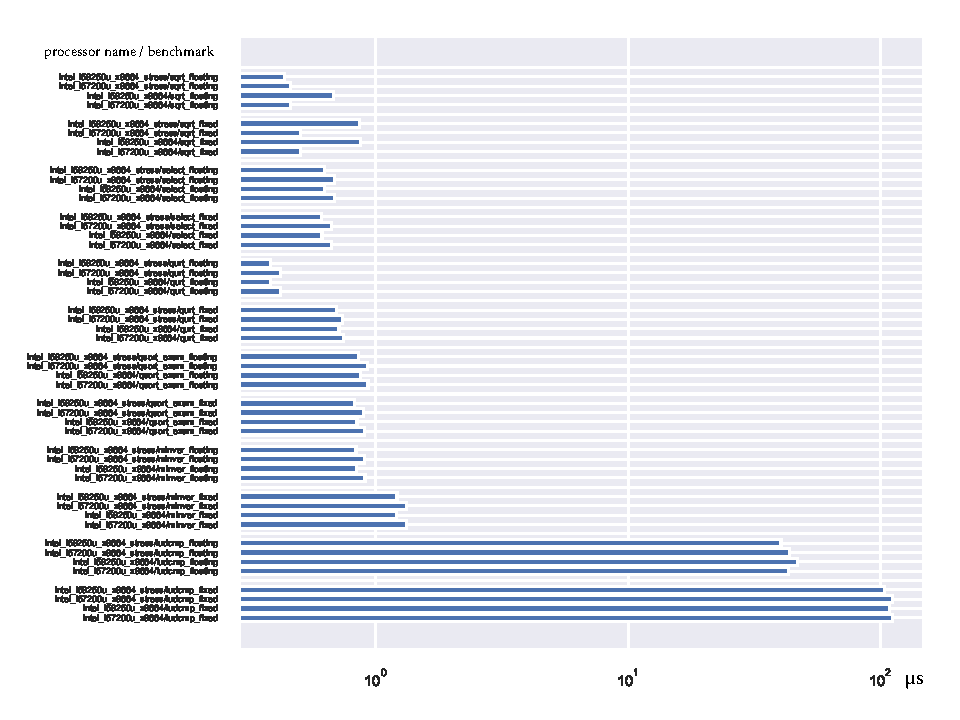
\includegraphics[width=565pt]{intel_mean_histogram.pdf}
\clearpage

\textbf{Smartphones armv8a mean histogram}\newline
\hspace*{-3.2cm}
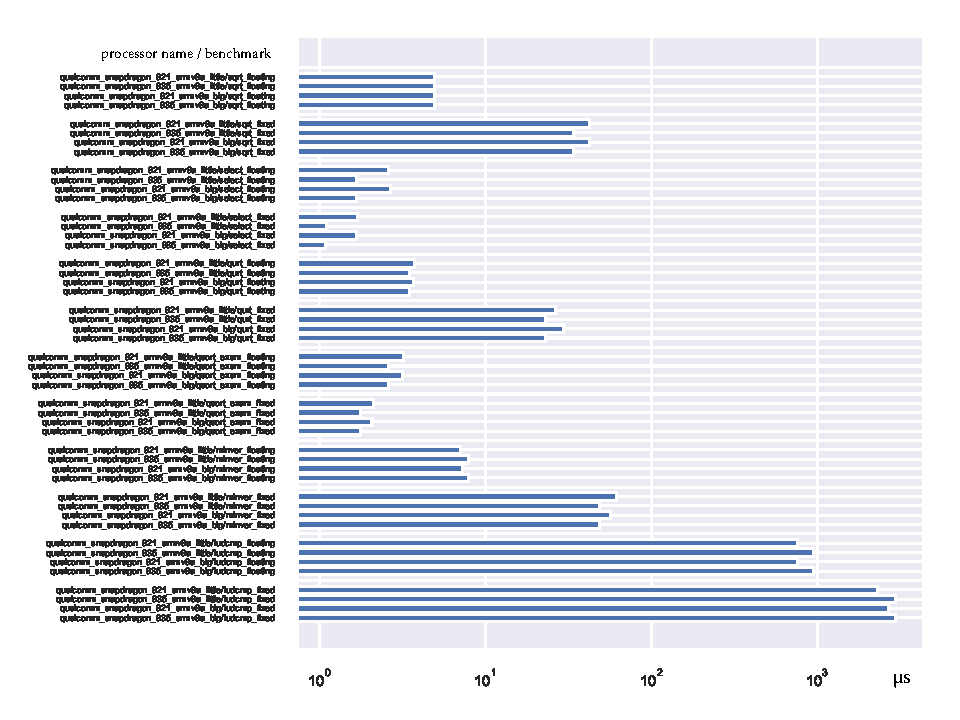
\includegraphics[width=570pt]{smartphones_mean_histogram.pdf}
\clearpage

\textbf{Freescale i.MX6 and ODROID XU3 mean histogram}\newline
\hspace*{-3.2cm}
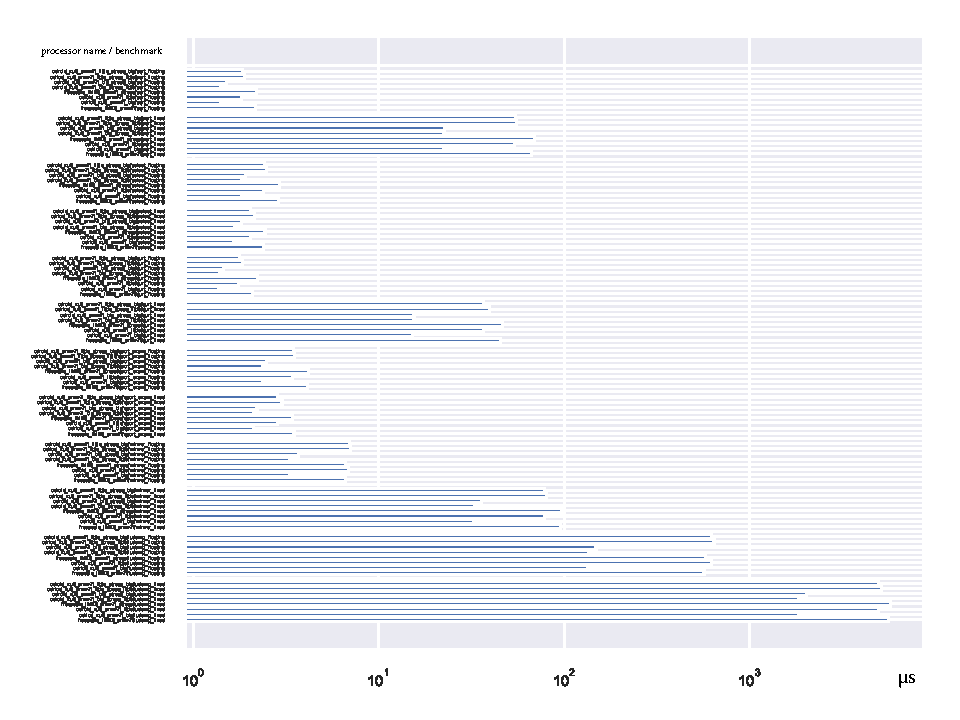
\includegraphics[width=570pt]{boards_mean_histogram.pdf}
\clearpage




\subsection{Standard Deviation}
Now a series of histograms are displayed to better comprehend the behaviour of the different architectures.
These histograms show the standard deviation expressed in microseconds for each benchmark and each processor.\newline
Note: that the x scale is logarithmic.\newline

\textbf{Intel x86\_64 standard deviation histogram}\newline
\hspace*{-3.2cm}
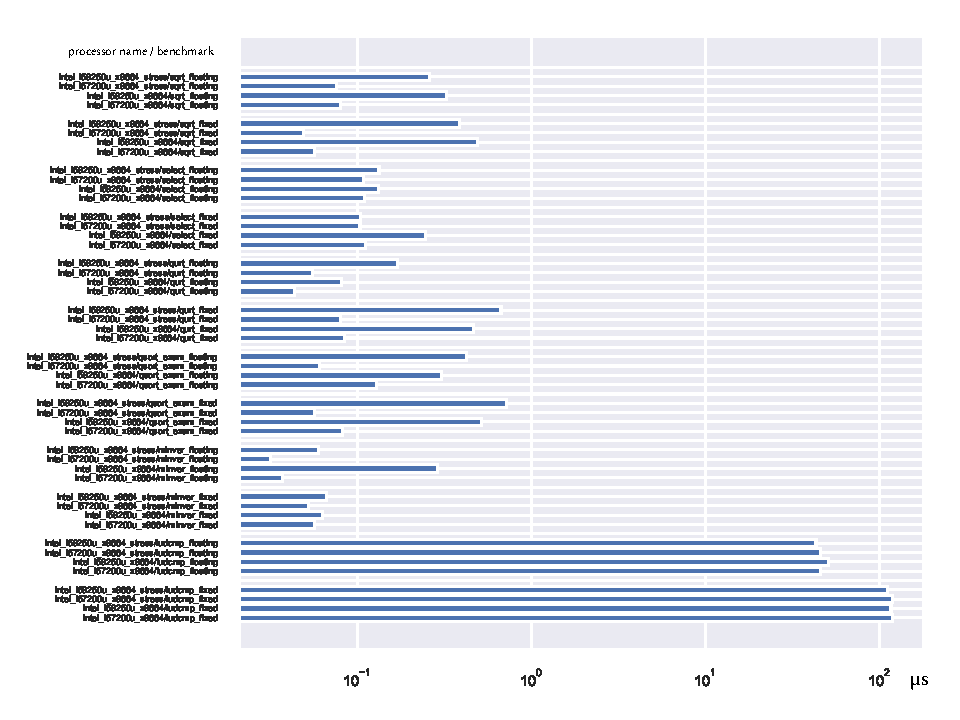
\includegraphics[width=570pt]{intel_stddev_histogram.pdf}
\clearpage
In the previous histogram we can identify the following singularities:
Comparing fixed point vs floating point operations:
\begin{itemize}
		\item In the benchmarks \textit{select}, \textit{qurt}, \textit{ludcmp} fixed point operations have a larger standard deviation.
		\item In the benchmarks \textit{sqrt}, \textit{qsort\_exam}, \textit{minver} we observe conflicting behaviours between the two processors (ex: in the \textit{qsort\_exam} benchmark the Intel i5 7200U has a lower standard deviation for the fixed point benchamark with respect to the floating point one. Instead the Intel i5 8250U has the opposite behaviour).
\end{itemize}
Comparing fixed point vs floating point operations with stress:
\begin{itemize}
		\item In the benchmarks \textit{qurt}, \textit{minver}, \textit{ludcmp} fixed point operations have a larger standard deviation.
		\item In the benchmark \textit{select} fixed point operations have a smaller standard deviation.
		\item In the benchmarks \textit{sqrt}, \textit{qsort\_exam} we observe conflicting behaviours between the two processors.
\end{itemize}

\clearpage
\textbf{Smartphones armv8a standard deviation histogram}\newline
\hspace*{-3.2cm}
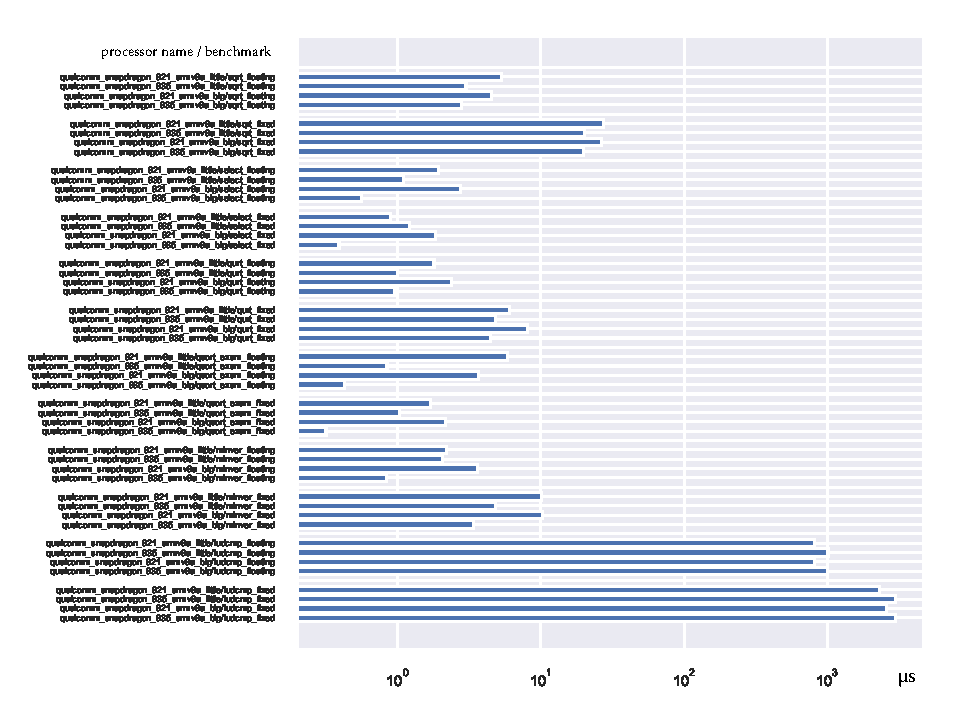
\includegraphics[width=570pt]{smartphones_stddev_histogram.pdf}
\clearpage
In the previous histogram we can identify the following singularities:
Comparing fixed point vs floating point operations on the big cluster:
\begin{itemize}
		\item In the benchmarks \textit{sqrt}, \textit{qurt}, \textit{minver}, \textit{ludcmp} fixed point operations have a larger standard deviation.
		\item In the benchmarks \textit{select}, \textit{qsort\_exam} fixed point operations have a smaller standard deviation.
\end{itemize}
Comparing fixed point vs floating point operations on the LITTLE cluster:
\begin{itemize}
		\item In the benchmarks \textit{sqrt}, \textit{qurt}, \textit{minver}, \textit{ludcmp} fixed point operations have a larger standard deviation.
		\item In the benchmarks \textit{select}, \textit{qsort\_exam} we observe conflicting behaviours between the two processors.
\end{itemize}

\clearpage
\textbf{Freescale i.MX 6 and ODROID XU3 standard deviation histogram}\newline
\hspace*{-3.2cm}
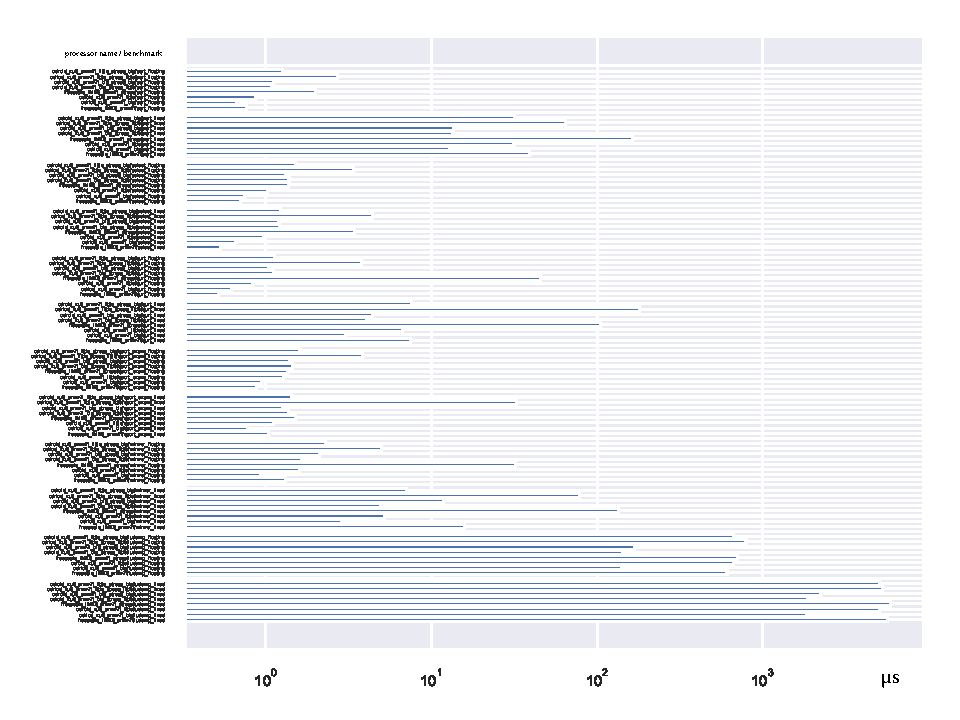
\includegraphics[width=570pt]{boards_stddev_histogram.pdf}
\clearpage
In the previous histogram we can identify the following singularities:
Comparing fixed point vs floating point operations on the Freescale i.MX 6 and the ODROID XU3 big and LITTLE cluster:
\begin{itemize}
		\item In the benchmarks \textit{sqrt}, \textit{qurt}, \textit{minver}, \textit{ludcmp} fixed point operations have a larger standard deviation.
		\item In the benchmark \textit{select} fixed point operations have a smaller standard deviation.
		\item In the benchmark \textit{qsort\_exam} we observe conflicting behaviours between the two processors (ODROID XU3 has lower standard deviation for fixed point operations, Freescale i.MX 6 has an higher standard deviation).
\end{itemize}
Comparing fixed point vs floating point operations with stress on the Freescale i.MX 6 and the ODRIOD XU3 big and LITTLE cluster:
\begin{itemize}
		\item In the benchmarks \textit{sqrt}, \textit{qurt}, \textit{minver}, \textit{ludcmp} fixed point operations have a larger standard deviation.
		\item In the benchmarks \textit{select}, \textit{qsort\_exam} we observe conflicting behaviours between the two processors (In the \textit{select} benchmark the ODROID XU3 running on the LITTLE cluster and stressed on this cluster has a higher standard deviation, the same for the Freescale i.MX 6 under stress. The exact same behaviour is observed with the benchmark \textit{qsort\_exam}).
\end{itemize}

\subsection{KPSS}
In the provided \href{../statistics/tests\_results.txt}{report} we can see that:
\begin{itemize}
	\item Out of 96 floating point benchmarks, 76 have passed the KPSS test with a 5\% significance level, so we cannot reject the null hypothesis H0.
	\item Out of 96 fixed point benchmarks, 68 have passed the KPSS test with a 5\% significance level, so we cannot reject the null hypothesis H0.
\end{itemize}
As we can see, an higher percentage of floating point benchmarks have passed the KPSS test, so the time series generated by floating point benchmarks have an higher probability of being stationary.\newline
Note: in the report there are also the results for 2.5\% and 1\% significance levels.

\subsection{BDS}
From the generated report, no benchmark has passed the BDS test. This was predictable, since we expected that the benchmarks results are not I.I.D..

\subsection{Hurst Exponent}
The Hurst Exponent is not a statistic test, but depending on the value a different behaviour can be identified on the time series.\newline
Range 0.5-1, positive autocorrelation:
\begin{itemize}
	\item Out of 96 floating point benchmarks, 86 have an Hurst Exponent in this range.
	\item Out of 96 fixed point benchmarks, 93 have an Hurst Exponent in this range.
\end{itemize}
There is no benchmark which have exactly 0.5 as Hurst Exponent, so in the range 0-0.5, in which the time-series have a long-term switching behaviour, the results are:
\begin{itemize}
	\item Out of 96 floating point benchmarks, 10 have an Hurst Exponent in this range.
	\item Out of 96 fixed point benchmarks, 3 have an Hurst Exponent in this range.
\end{itemize}

We can conclude that fixed point benchmarks measurements have an higher probability to compose a time series with a long-term positive autocorrelation.
\clearpage
\section{Conclusions}
It is needed to differentiate the set of benchmarks, because depending on the complexity of the benchmark floating point operations are more predictable with respect to fixed point operations.\newline
We have to take into account that our implementations of multiplication and division, in both 128-bit supported and not supported version, guarantee a quite high level of precision.
To support such an high level of precision we had to use 128-bit registers or complex procedures, that affect both performance and predictability of fixed point benchmarks. We assume that if a lower level of precision is acceptable fixed point benchmarks would have produced better results on computing intensive benchmarks.
 
\subsection{Computing intensive benchmarks}
We identified two benchmarks, \textit{qurt} and \textit{ludcmp}, that execute a large number of divisions and multiplications; in these benchmarks the fixed point versions have always an higher standard deviation and lower performances with respect to their floating point version, under every circumstance (platform, cluster and stress).
Instead, \textit{sqrt} and \textit{minver} benchmarks are also computing intensive but in this case often, but not always, the fixed point versions have an higher standard deviation and lower performances.

\subsection{Light computing benchmarks}
We identified two benchmarks, \textit{qsort\_exam} and \textit{select}, that do not execute any divisions or multiplications between fixed or floating point values; in these benchmarks the fixed point versions have often a lower standard deviation and always higher performances with respect to their floating point versions.\newline
We assume that addition and subtraction is less demanding and then more predictable between integers.

\subsection{Statistics tests \& Hurst Exponent}
Different considerations hold for statistics tests, as said before, no benchmark accepted the null hypothesis of the BDS test, so there is no time series in which the data are I.I.D., as expected.
Moreover, the Hurst Exponent have highlighted that fixed point benchmarks have an higher probability of generating a time-series in which the consecutive values are similar between them. This implies that given a sample of the time-series we have an higher probability to predict the next sample in fixed point benchmarks.\newline
Finally, KPSS test null hypothesis was rejected by more fixed point benchmarks than floating point benchmarks, so we can assume that there is an higher probability of generating a stationary time-series when using a floating-point benchmark.

\end{document}